         \chapter{The atom}
    \setcounter{figure}{1}
    \setcounter{subfigure}{1}
    \label{ea1c9e59656f96ee804546971cf6dee6}
         \section{ Introduction and models}
    \nopagebreak
            \label{m38756} $ \hspace{-5pt}\begin{array}{cccccccccccc}   
\includegraphics[width=0.75cm]{col11305.imgs/summary_video.png} &   \end{array} $ \hspace{2 pt}\raisebox{-5 pt}{} {(section shortcode: P10019 )} \par 
    \label{m38756*cid1}
            \subsection{ Introduction}
            \nopagebreak
      \label{m38756*eip-794}The following video covers some of the properties of an atom.
    \setcounter{subfigure}{0}
	\begin{figure}[H] % horizontal\label{m38756*the-atom-1}
    \textnormal{Veritasium video on the atom - 1}\vspace{.1in} \nopagebreak
  \label{m38756*yt-media10}\label{m38756*yt-video10}
            \raisebox{-5 pt}{ 
\includegraphics[width=0.5cm]{col11305.imgs/summary_www.png}} { (Video:  P10020 )}
      \vspace{2pt}
    \vspace{.1in}
 \end{figure}       \par \label{m38756*id254141}We have now looked at many examples of the types of matter and materials that exist around us and we have investigated some of the ways that materials are classified. But what is it that makes up these materials? And what makes one material different from another? In order to understand this, we need to take a closer look at the building block of matter - the \textbf{atom}. Atoms are the basis of all the structures and organisms in the universe. The planets, sun, grass, trees, air we breathe and people are all made up of different combinations of atoms.\par 
    \label{m38756*eip-613}
            \subsection{ Project: Models of the atom}
            \nopagebreak
            \label{m38756*eip-3}
Our current understanding of the atom came about over a long period of time, with many different people playing a role. Conduct some research into the development of the different ideas of the atom and the people who contributed to it. Some suggested people to look at are: JJ Thomson, Ernest Rutherford, Marie Curie, JC Maxwell, Max Planck, Albert Einstein, Niels Bohr, Lucretius, LV de Broglie, CJ Davisson, LH Germer, Chadwick, Werner Heisenberg, Max Born, Erwin Schrodinger, John Dalton, Empedocles, Leucippus, Democritus, Epicurus, Zosimos, Maria the Jewess, Geber, Rhazes, Robert Boyle, Henry Cavendish, A Lavoisier and H Becquerel. You do not need to find information on all these people, but try to find information about as many of them as possible.
\par 
\label{m38756*id7342}Make a list of the key contributions to a model of the atom that each of these people made and then make a timeline of this information. (You can use an online tool such as Dipity\footnote{http://www.dipity.com/}
         to make a timeline.) Try to get a feel for how it all eventually fit together into the modern understanding of the atom. 
\par \label{m38756*cid2}
            \subsection{ Models of the Atom}
            \nopagebreak
      \label{m38756*id254164}It is important to realise that a lot of what we know about the structure of atoms has been developed over a long period of time. This is often how scientific knowledge develops, with one person building on the ideas of someone else. We are going to look at how our modern understanding of the atom has evolved over time.\par 
      \label{m38756*id254508}The idea of atoms was invented by two Greek philosophers, Democritus and Leucippus in the fifth century BC. The Greek word $\mathrm{\alpha \tau o\mu o\nu }$ \hspace{1ex} (atom) means \textbf{indivisible} because they believed that atoms could not be broken into smaller pieces.\par 
      \label{m38756*id254540}Nowadays, we know that atoms are made up of a \textbf{positively charged nucleus} in the centre
surrounded by \textbf{negatively charged electrons}. However, in the past, before the structure of the atom was properly understood, scientists came up with lots of different \textbf{models} or \textbf{pictures} to describe what atoms look like.\par 
\label{m38756*fhsst!!!underscore!!!id72}\begin{definition}
	  \begin{tabular*}{15 cm}{m{15 mm}m{}}
	\hspace*{-50pt}  
\includegraphics[width=0.5in]{col11305.imgs/psflag2.png}   & \Definition{   \label{id2414493}\textbf{ Model }} { \label{m38756*meaningfhsst!!!underscore!!!id72}
      \label{m38756*id254584}A model is a representation of a system in the real world. Models help us to understand systems and their properties. For example, an \textsl{atomic model} represents what the structure of an atom \textsl{could} look like, based on what we know about how atoms behave. It is not necessarily a true picture of the exact structure of an atom. \par 
       } 
      \end{tabular*}
      \end{definition}
      \label{m38756*uid1}
            \subsubsection{ The Plum Pudding Model}
            \nopagebreak
        \label{m38756*id254616}After the electron was discovered by J.J. Thomson in 1897, people realised that atoms were made up of even smaller particles than they had previously thought. However, the atomic nucleus had not been discovered yet and so the 'plum pudding model' was put forward in 1904. In this model, the atom is made up of negative electrons that float in a soup of positive charge, much like plums in a pudding or raisins in a fruit cake (Figure~3.2). In 1906, Thomson was awarded the Nobel Prize for his work in this field. However, even with the Plum Pudding Model, there was still no understanding of how these electrons in the atom were arranged.\par 
    \setcounter{subfigure}{0}
	\begin{figure}[H] % horizontal\label{m38756*uid2}
    \begin{center}
    \rule[.1in]{\figurerulewidth}{.005in} \\
        \label{m38756*uid2!!!underscore!!!media}\label{m38756*uid2!!!underscore!!!printimage}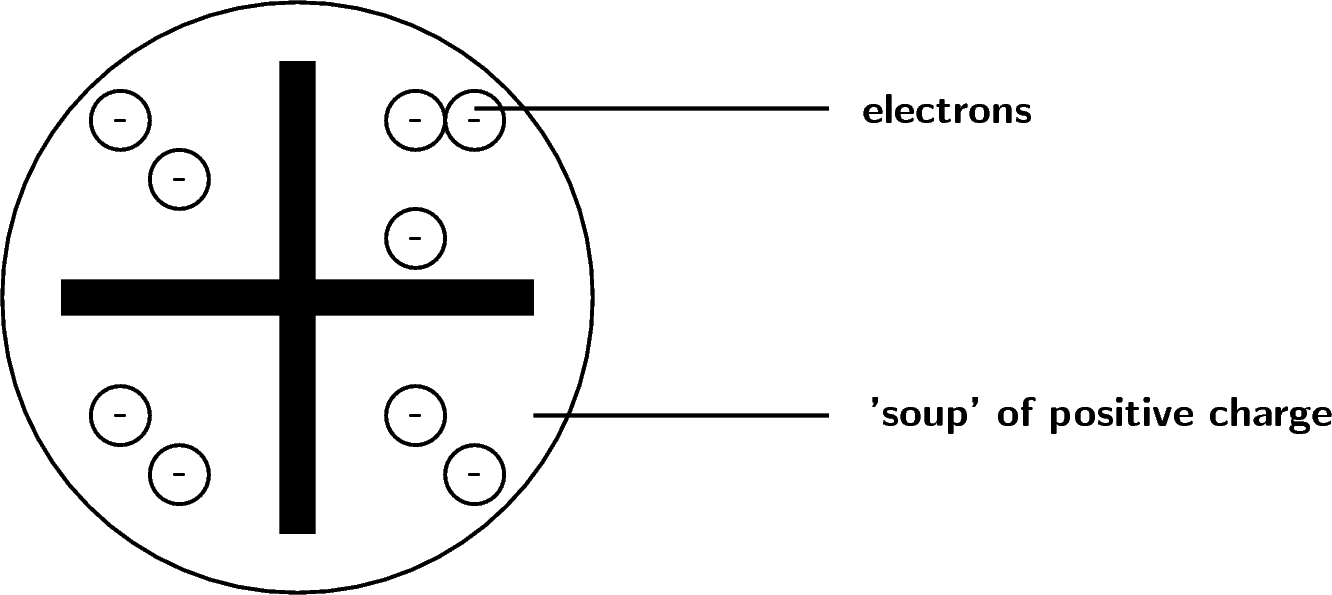
\includegraphics[width=9cm]{col11305.imgs/m38756_CG10C3_001.png} % m38756;CG10C3\_001.png;;;6.0;8.5;
      \vspace{2pt}
    \vspace{\rubberspace}\par \begin{cnxcaption}
	  \small \textbf{Figure 3.2: }A schematic diagram to show what the atom looks like according to the Plum Pudding model
	\end{cnxcaption}
    \vspace{.1in}
    \rule[.1in]{\figurerulewidth}{.005in} \\
    \end{center}
 \end{figure}       
        \label{m38756*id254642}The discovery of \textbf{radiation} was the next step along the path to building an accurate picture of atomic structure. In the early twentieth century, Marie Curie and her husband Pierre,  discovered that some elements (the \textsl{radioactive} elements) emit particles, which are able to pass through matter in a similar way to X-rays (read more about this in Grade 11). It was Ernest Rutherford who, in 1911, used this discovery to revise the model of the atom.\par 
      \label{m38756*eip-956}
\begin{tabular}{cc}
	\hspace*{-50pt}\raisebox{-8 mm}{\hspace{-0.2in}
\includegraphics[width=0.75in]{col11305.imgs/psfact2.png} } & 
	\begin{minipage}{0.85\textwidth}
	\begin{note}
      {note: }Two other models proposed for the atom were the cubic model and the Saturnian model. In the cubic model, the electrons were imagined to lie at the corners of a cube. In the Saturnian model, the electrons were imagined to orbit a very big, heavy nucleus.
	\end{note}
	\end{minipage}
	\end{tabular}
	\par
      \label{m38756*uid3}
            \subsubsection{ Rutherford's model of the atom}
            \nopagebreak
            \label{m38756*id254751}Rutherford carried out some experiments which led to a change in ideas around the atom. His new model described the atom as a tiny, dense, positively charged core called a nucleus surrounded by lighter, negatively charged electrons. Another way of thinking about this model was that the atom was seen to be like a mini solar system where the electrons orbit the nucleus like planets orbiting around the sun. A simplified picture of this is shown in Figure~3.3. This model is sometimes known as the planetary model of the atom.\par 
    \setcounter{subfigure}{0}
	\begin{figure}[H] % horizontal\label{m38756*uid5}
    \begin{center}
    \rule[.1in]{\figurerulewidth}{.005in} \\
        \label{m38756*uid5!!!underscore!!!media}\label{m38756*uid5!!!underscore!!!printimage}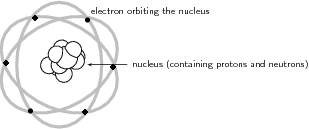
\includegraphics[width=8cm]{col11305.imgs/m38756_CG10C3_003.png} % m38756;CG10C3\_003.png;;;6.0;8.5;
      \vspace{2pt}
    \vspace{\rubberspace}\par \begin{cnxcaption}
	  \small \textbf{Figure 3.3: }Rutherford's model of the atom
	\end{cnxcaption}
    \vspace{.1in}
    \rule[.1in]{\figurerulewidth}{.005in} \\
    \end{center}
 \end{figure}       
      \label{m38756*uid6}
            \subsubsection{ The Bohr Model}
            \nopagebreak
        \label{m38756*id254784}There were, however, some problems with this model: for example it could not explain the very interesting
observation that atoms only emit light at certain wavelengths or frequencies. Niels Bohr solved
this problem by proposing that the electrons could only orbit the nucleus in certain special orbits
at different energy levels around the nucleus. The exact energies of the orbitals in each energy level depends on
the type of atom. Helium for example, has different energy levels to Carbon. If an electron jumps down
from a higher energy level to a lower energy level, then light is emitted from
the atom. The energy of the light emitted is the same as the gap in the energy between the two
energy levels. You can read more about this in "Energy quantisation and electron configuration". The distance between the nucleus and the electron in the lowest energy level of a hydrogen atom is known as the \textbf{Bohr radius}.\par 
\label{m38756*notfhsst!!!underscore!!!id119}
\begin{tabular}{cc}
	\hspace*{-50pt}\raisebox{-8 mm}{\hspace{-0.2in}
\includegraphics[width=0.75in]{col11305.imgs/psfact2.png} } & 
	\begin{minipage}{0.85\textwidth}
	\begin{note}
      {note: }
        \label{m38756*id254816}Light has the properties of both a particle \textbf{and} a wave! Einstein discovered
that light comes in energy packets which are called \textbf{photons}. When an electron in an atom
changes energy levels, a photon of light is emitted. This photon has the same energy as
the difference between the two electron energy levels.\par 
	\end{note}
	\end{minipage}
	\end{tabular}
	\par
      \label{m38756*eip-279}
            \subsubsection{ Other models of the atom}
            \nopagebreak
            \label{m38756*eip-993}
Although the most common model of the atom is the Bohr model, scientists have not stopped thinking about other ways to describe atoms. One of the most important contributions to atomic theory (the field of science that looks at atoms) was the development of quantum theory. Schrodinger, Heisenberg, Born and many others have had a role in developing quantum theory. The description of an atom by quantum theory is very complex and is only covered at university level.  
\par \label{m38756*eip-179}
            \subsubsection{ Models of the atom}
            \nopagebreak
            \label{m38756*eip-786}Match the information in column A, with the key discoverer in column B.
    % \textbf{m38756*eip-551}\par
          \begin{table}[H]
    % \begin{table}[H]
    % \\ '' '0'
        \begin{center}
      \label{m38756*eip-551}
    \noindent
    \tabletail{%
        \hline
        \multicolumn{2}{|p{\mytableboxwidth}|}{\raggedleft \small \sl continued on next page}\\
        \hline
      }
      \tablelasttail{}
      \begin{xtabular}[t]{|l|l|}\hline
        Column A &
        Column B% make-rowspan-placeholders
     \tabularnewline\cline{1-1}\cline{2-2}
      %--------------------------------------------------------------------
        Discovery of electrons and the plum pudding model &
        Niels Bohr% make-rowspan-placeholders
     \tabularnewline\cline{1-1}\cline{2-2}
      %--------------------------------------------------------------------
        Arrangement of electrons &
        Marie Curie and her husband, Pierre% make-rowspan-placeholders
     \tabularnewline\cline{1-1}\cline{2-2}
      %--------------------------------------------------------------------
        Atoms as the smallest building block of matter &
        Ancient Greeks% make-rowspan-placeholders
     \tabularnewline\cline{1-1}\cline{2-2}
      %--------------------------------------------------------------------
        Discovery of the nucleus &
        JJ Thomson% make-rowspan-placeholders
     \tabularnewline\cline{1-1}\cline{2-2}
      %--------------------------------------------------------------------
        Discovery of radiation &
        Rutherford% make-rowspan-placeholders
     \tabularnewline\cline{1-1}\cline{2-2}
      %--------------------------------------------------------------------
    \end{xtabular}
      \end{center}
    \begin{center}{\small\bfseries Table 3.1}\end{center}
    \begin{caption}{\small\bfseries Table 3.1}\end{caption}
\end{table}
    \par
        \par 
    \label{m38756*cid3}
\par \raisebox{-5 pt}{
\includegraphics[width=0.5cm]{col11305.imgs/summary_www.png}} Find the answers with the shortcodes:
 \par \begin{tabular}[h]{cccccc}
 (1.) l4g  & \end{tabular}
            \subsection{ Atomic mass and diameter}
            \nopagebreak
            \label{m38756*id254850}It is difficult sometimes to imagine the size of an atom, or its mass, because we cannot see an atom and also because we are not used to working with such small measurements.\par 
      \label{m38756*uid7}
            \subsubsection{ How heavy is an atom?}
            \nopagebreak
        \label{m38756*id254863}It is possible to determine the mass of a single atom in kilograms. But to do this, you would need very modern \textsl{mass spectrometers} and the values you would get would be very clumsy and difficult to use. The mass of a carbon atom, for example, is about $1,99\ensuremath{\times}{10}^{-26}\phantom{\rule{2pt}{0ex}}\mathrm{kg}$, while the mass of an atom of hydrogen is about $1,67\ensuremath{\times}{10}^{-27}\phantom{\rule{2pt}{0ex}}\mathrm{kg}$. Looking at these very small numbers makes it difficult to compare how much bigger the mass of one atom is when compared to another.\par 
        \label{m38756*id254908}To make the situation simpler, scientists use a different unit of mass when they are describing the mass of an atom. This unit is called the \textbf{atomic mass unit} (amu). We can abbreviate (shorten) this unit to just 'u'. Scientists use the \textbf{carbon standard} to determine amu. The carbon standard assigns carbon an atomic mass of 12 u. Using the carbon standard the mass of an atom of hydrogen will be 1 u. You can check this by dividing the mass of a carbon atom in kilograms (see above) by the mass of a hydrogen atom in kilograms (you will need to use a calculator for this!). If you do this calculation, you will see that the mass of a carbon atom is twelve times greater than the mass of a hydrogen atom. When we use atomic mass units instead of kilograms, it becomes easier to see this. Atomic mass units are therefore not giving us the \textsl{actual} mass of an atom, but rather its mass \textsl{relative} to the mass of one (carefully chosen) atom in the Periodic Table. Although carbon is the usual element to compare other elements to, oxygen and hydrogen have also been used. The important thing to remember here is that the atomic mass unit is relative to one (carefully chosen) element. The atomic masses of some elements are shown in the  table  (Table 3.2) below.\par 
    % \textbf{m38756*uid8}\par
          \begin{table}[H]
    % \begin{table}[H]
    % \\ '' '0'
        \begin{center}
      \label{m38756*uid8}
    \noindent
    \tabletail{%
        \hline
        \multicolumn{2}{|p{\mytableboxwidth}|}{\raggedleft \small \sl continued on next page}\\
        \hline
      }
      \tablelasttail{}
      \begin{xtabular}[t]{|l|l|}\hline
                  \textbf{Element}
                 &
                  \textbf{Atomic mass (u)}
                % make-rowspan-placeholders
     \tabularnewline\cline{1-1}\cline{2-2}
      %--------------------------------------------------------------------
        Carbon ($\mathrm{C}$) &
        12% make-rowspan-placeholders
     \tabularnewline\cline{1-1}\cline{2-2}
      %--------------------------------------------------------------------
        Nitrogen ($\mathrm{N}$) &
        14% make-rowspan-placeholders
     \tabularnewline\cline{1-1}\cline{2-2}
      %--------------------------------------------------------------------
        Bromine ($\mathrm{Br}$) &
        80% make-rowspan-placeholders
     \tabularnewline\cline{1-1}\cline{2-2}
      %--------------------------------------------------------------------
        Magnesium ($\mathrm{Mg}$) &
        24% make-rowspan-placeholders
     \tabularnewline\cline{1-1}\cline{2-2}
      %--------------------------------------------------------------------
        Potassium ($\mathrm{K}$) &
        39% make-rowspan-placeholders
     \tabularnewline\cline{1-1}\cline{2-2}
      %--------------------------------------------------------------------
        Calcium ($\mathrm{Ca}$) &
        40% make-rowspan-placeholders
     \tabularnewline\cline{1-1}\cline{2-2}
      %--------------------------------------------------------------------
        Oxygen ($\mathrm{O}$) &
        16% make-rowspan-placeholders
     \tabularnewline\cline{1-1}\cline{2-2}
      %--------------------------------------------------------------------
    \end{xtabular}
      \end{center}
    \begin{center}{\small\bfseries Table 3.2}: The atomic mass number of some of the elements\end{center}
    \begin{caption}{\small\bfseries Table 3.2}: The atomic mass number of some of the elements\end{caption}
\end{table}
    \par
        \label{m38756*id255096}The actual value of 1 atomic mass unit is $1,67\ensuremath{\times}{10}^{-24}\phantom{\rule{2pt}{0ex}}\mathrm{g}$ or $1,67\ensuremath{\times}{10}^{-27}\phantom{\rule{2pt}{0ex}}\mathrm{kg}$. This is a very tiny mass!\par 
      \label{m38756*uid9}
            \subsubsection{ How big is an atom?}
            \nopagebreak
\label{m38756*notfhsst!!!underscore!!!id177}
\begin{tabular}{cc}
	   \hspace*{-50pt}\raisebox{-8 mm}{ 
\includegraphics[width=0.5in]{col11305.imgs/pstip2.png}  }& 
	\begin{minipage}{0.85\textwidth}
	\begin{note}
      {tip: }\textsl{pm} stands for \textsl{picometres}. $1\phantom{\rule{2pt}{0ex}}\mathrm{pm}={10}^{-12}\phantom{\rule{2pt}{0ex}}\mathrm{m}$
	\end{note}
	\end{minipage}
	\end{tabular}
	\par
        \label{m38756*id255173}Atomic radius also varies depending on the element. On average, the radius of an atom ranges from $32\phantom{\rule{2pt}{0ex}}\mathrm{pm}$ (Helium) to $225\phantom{\rule{2pt}{0ex}}\mathrm{pm}$ (Caesium). Using different units, $100\phantom{\rule{2pt}{0ex}}\mathrm{pm}=1\phantom{\rule{2pt}{0ex}}\mathrm{Angstrom}$, and $1\phantom{\rule{2pt}{0ex}}\mathrm{Angstrom}={10}^{-10}\phantom{\rule{2pt}{0ex}}\mathrm{m}$. That is the same as saying that $1\phantom{\rule{2pt}{0ex}}\mathrm{Angstrom}=0,0000000010\phantom{\rule{2pt}{0ex}}\mathrm{m}$ or that $100\phantom{\rule{2pt}{0ex}}\mathrm{pm}=0,0000000010\phantom{\rule{2pt}{0ex}}\mathrm{m}$! In other words, the diameter of an atom ranges from $0,0000000010\phantom{\rule{2pt}{0ex}}m$ to $0,0000000067\phantom{\rule{2pt}{0ex}}m$. This is very small indeed.\par \label{m38756*eip-30}The atomic radii given above are for the whole atom (nucleus and electrons). The nucleus itself is even smaller than this by a factor of about 23 000 in uranium and 145 000 in hydrogen. If the nucleus were the size of a golf ball, then the nearest electrons would be about one kilometer away! This should help you realise that the atom is mostly made up of empty space. \par \label{m38756*eip-320}
            \subsubsection{ Rutherfords alpha-particle scattering experiment}
            \nopagebreak
            \label{m38756*id254668}Radioactive elements emit different types of particles. Some of these are positively charged alpha ($\alpha $) particles.
Rutherford carried out a series of experiments where he bombarded sheets of gold foil with these particles, to try to get a better understanding of where the positive charge in the atom was. A simplified diagram of his experiment is shown in Figure~3.4.\par 
    \setcounter{subfigure}{0}
	\begin{figure}[H] % horizontal\label{m38756*uid4}
    \begin{center}
    \rule[.1in]{\figurerulewidth}{.005in} \\
        \label{m38756*uid4!!!underscore!!!media}\label{m38756*uid4!!!underscore!!!printimage}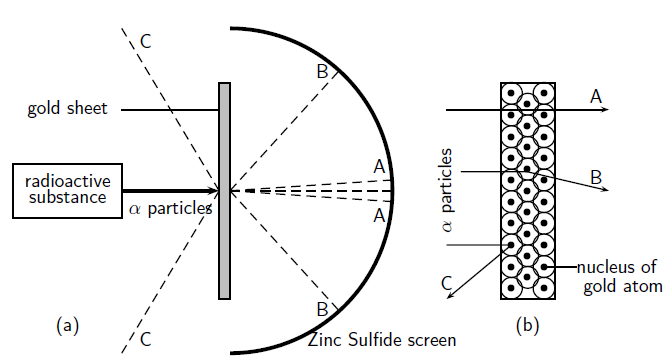
\includegraphics[width=300px]{col11305.imgs/m38756_CG10C3_002.png} % m38756;CG10C3\_002.png;;;6.0;8.5;
      \vspace{2pt}
    \vspace{\rubberspace}\par \begin{cnxcaption}
	  \small \textbf{Figure 3.4: }Rutherford's gold foil experiment. Figure (a) shows the path of the $\alpha $ particles after they hit the gold sheet. Figure (b) shows the arrangement of atoms in the gold sheets and the path of the $\alpha $ particles in relation to this.
	\end{cnxcaption}
    \vspace{.1in}
    \rule[.1in]{\figurerulewidth}{.005in} \\
    \end{center}
 \end{figure}       
        \label{m38756*id254715}Rutherford set up his experiment so that a beam of alpha particles was directed at the gold sheets. Behind the gold sheets was a screen made of zinc sulphide. This screen allowed Rutherford to see where the alpha particles were landing. Rutherford knew that the \textsl{electrons} in the gold atoms would not really affect the path of the alpha particles, because the mass of an electron is so much smaller than that of a proton. He reasoned that the positively charged \textsl{protons} would be the ones to \textsl{repel} the positively charged alpha particles and alter their path.\par 
        \label{m38756*id254738}What he discovered was that most of the alpha particles passed through the foil undisturbed and could be detected on the screen directly behind the foil (A). Some of the particles ended up being slightly deflected onto other parts of the screen (B). But what was even more interesting was that some of the particles were deflected straight back in the direction from where they had come (C)! These were the particles that had been repelled by the positive protons in the gold atoms. If the Plum Pudding model of the atom were true then Rutherford would have expected much more repulsion, since the positive charge according to that model is distributed throughout the atom. But this was not the case. The fact that most particles passed straight through suggested that the positive charge was concentrated in one part of the atom only.\par 
      \label{m38756*eip-491}
            \subsubsection{ Relative atomic mass}
            \nopagebreak
            \par
            \label{m38756*eip-890}\begin{definition}
	  \begin{tabular*}{15 cm}{m{15 mm}m{}}
	\hspace*{-50pt}  
\includegraphics[width=0.5in]{col11305.imgs/psflag2.png}   & \Definition{   \label{id2415700}\textbf{ Relative atomic mass }} { \label{m38756*meaningfhsst!!!underscore!!!id598}
        \label{m38756*id258580}Relative atomic mass is the average mass of one atom of all the naturally occurring isotopes of a particular chemical element, expressed in atomic mass units.
 \par 
         } 
      \end{tabular*}
      \end{definition}
\label{m38756*eip-933}The relative atomic mass of an element is the number you will find on the periodic table. \par 
  \label{m38756**end}
         \section{ Structure}
    \nopagebreak
            \label{m38745} $ \hspace{-5pt}\begin{array}{cccccccccccc}   
\includegraphics[width=0.75cm]{col11305.imgs/summary_fullmarks.png} &   \end{array} $ \hspace{2 pt}\raisebox{-5 pt}{} {(section shortcode: P10021 )} \par 
    \label{m38745*cid4}
            \subsection{ Structure of the atom}
            \nopagebreak
      \label{m38745*id255206}As a result of the work done by previous scientists on atomic models (that we discussed in "Models of the Atom"), scientists now have a good idea of what an atom looks like. This knowledge is important because it helps us to understand why materials have different properties and why some materials bond with others. Let us now take a closer look at the microscopic structure of the atom.\par 
      \label{m38745*id255216}So far, we have discussed that atoms are made up of a positively charged \textbf{nucleus} surrounded by
one or more negatively charged \textbf{electrons}. These electrons orbit the nucleus.\par 
      \label{m38745*eip-577}Before we look at some useful concepts we first need to understand what electrons, protons and neutrons are.\par \label{m38745*uid10}
            \subsubsection{ The Electron}
            \nopagebreak
        \label{m38745*id255241}The electron is a very light particle. It has a mass of $9,11\ensuremath{\times}{10}^{-31}\phantom{\rule{2pt}{0ex}}\mathrm{kg}$.
Scientists believe that the electron can be treated as a \textbf{point particle}
or \textbf{elementary particle}
meaning that it can't be broken down into anything smaller. The electron also carries one unit
of \textbf{negative} electric charge which is the same as $1,6\ensuremath{\times}{10}^{-19}\phantom{\rule{2pt}{0ex}}\mathrm{C}$ (Coulombs).\par \label{m38745*eip-222}The electrons determine the charge on an atom. If the number of electrons is the same as the number of protons then the atom will be neutral. If the number of electrons is greater than the number of protons then the atom will be negatively charged. If the number of electrons is less than the number of protons then the atom will be positively charged. Atoms that are not neutral are called ions. Ions will be covered in more detail in a later chapter. For now all you need to know is that for each electron you remove from an atom you loose $-1$ of charge and for each electron that you add to an atom you gain $+1$ of charge. For example, the charge on an atom of sodium after removing one electron is  $-1$.\par 
      \label{m38745*uid11}
            \subsubsection{ The Nucleus}
            \nopagebreak
        \label{m38745*id255305}Unlike the electron, the nucleus \textbf{can} be broken up into smaller building
blocks called \textbf{protons} and \textbf{neutrons}. Together, the protons and
neutrons are called \textbf{nucleons}.\par 
        \label{m38745*uid12}
            \subsubsection{ The Proton}
            \nopagebreak
          \label{m38745*id255338}Each proton carries one unit of \textbf{positive} electric charge.
Since we know that atoms are
\textbf{electrically neutral}, i.e. do not carry any extra charge, then the number
of protons in an atom has to be the same as the number of electrons to balance
out the positive and negative charge to zero. The total positive charge of a
nucleus is equal to the number of protons in the nucleus. The proton is much heavier
than the electron (10 000 times heavier!) and has a mass of $1,6726\ensuremath{\times}{10}^{-27}\phantom{\rule{2pt}{0ex}}\mathrm{kg}$. When we talk about the atomic mass of an atom, we are mostly referring to the combined mass of the protons and neutrons, i.e. the nucleons.\par 
        \label{m38745*uid13}
            \subsubsection{ The Neutron}
            \nopagebreak
          \label{m38745*id254468}The neutron is electrically neutral i.e. it carries no charge at all.
Like the proton, it is much heavier than the electron and its mass is $1,6749\ensuremath{\times}{10}^{-27}\phantom{\rule{2pt}{0ex}}\mathrm{kg}$ (slightly heavier than the proton).\par 
\label{m38745*notfhsst!!!underscore!!!id214}
\begin{tabular}{cc}
	\hspace*{-50pt}\raisebox{-8 mm}{\hspace{-0.2in}
\includegraphics[width=0.75in]{col11305.imgs/psfact2.png} } & 
	\begin{minipage}{0.85\textwidth}
	\begin{note}
      {note: }
          \label{m38745*id254497}Rutherford predicted (in 1920) that another kind of particle must be
present in the nucleus along with the proton. He predicted this because
if there were only positively charged protons in the nucleus, then it should break
into bits because of the repulsive forces between the like-charged protons! Also,
if protons were the only particles
in the nucleus, then a helium nucleus (atomic number 2) would have
two protons and therefore only twice the mass of hydrogen. However,
it is actually \textbf{four} times heavier than hydrogen. This suggested that there
must be something else inside the nucleus as well as the protons.
To make sure that the atom stays electrically neutral, this particle would have to be neutral itself. In 1932 James Chadwick discovered the neutron and measured
its mass.\par 
	\end{note}
	\end{minipage}
	\end{tabular}
	\par
    % \textbf{m38745*uid14}\par
          \begin{table}[H]
    % \begin{table}[H]
    % \\ '' '0'
        \begin{center}
      \label{m38745*uid14}
    \noindent
    \tabletail{%
        \hline
        \multicolumn{4}{|p{\mytableboxwidth}|}{\raggedleft \small \sl continued on next page}\\
        \hline
      }
      \tablelasttail{}
      \begin{xtabular}[t]{|l|l|l|l|}\hline
         &
                    \textbf{proton}
                   &
                    \textbf{neutron}
                   &
                    \textbf{electron}
                  % make-rowspan-placeholders
     \tabularnewline\cline{1-1}\cline{2-2}\cline{3-3}\cline{4-4}
      %--------------------------------------------------------------------
                    \textbf{Mass (kg)}
                   &
        $1,6726\ensuremath{\times}{10}^{-27}$ &
        $1,6749\ensuremath{\times}{10}^{-27}$ &
        $9,11\ensuremath{\times}{10}^{-31}$% make-rowspan-placeholders
     \tabularnewline\cline{1-1}\cline{2-2}\cline{3-3}\cline{4-4}
      %--------------------------------------------------------------------
                    \textbf{Units of charge}
                   &
        $+1$ &
        $0$ &
        $-1$% make-rowspan-placeholders
     \tabularnewline\cline{1-1}\cline{2-2}\cline{3-3}\cline{4-4}
      %--------------------------------------------------------------------
                    \textbf{Charge (C)}
                   &
        $1,6\ensuremath{\times}{10}^{-19}$ &
        $0$ &
        $-1,6\ensuremath{\times}{10}^{-19}$% make-rowspan-placeholders
     \tabularnewline\cline{1-1}\cline{2-2}\cline{3-3}\cline{4-4}
      %--------------------------------------------------------------------
    \end{xtabular}
      \end{center}
    \begin{center}{\small\bfseries Table 3.3}: Summary of the particles inside the atom\end{center}
    \begin{caption}{\small\bfseries Table 3.3}: Summary of the particles inside the atom\end{caption}
\end{table}
    \par
    \label{m38745*cid5}
            \subsection{ Atomic number and atomic mass number}
            \nopagebreak
      \label{m38745*id255805}The chemical properties of an element are determined by the charge of
its nucleus, i.e. by the \textbf{number of protons}. This number is
called the \textbf{atomic number} and is denoted by the letter \textbf{Z}.\par 
\label{m38745*fhsst!!!underscore!!!id284}\begin{definition}
	  \begin{tabular*}{15 cm}{m{15 mm}m{}}
	\hspace*{-50pt}  
\includegraphics[width=0.5in]{col11305.imgs/psflag2.png}   & \Definition{   \label{id2416514}\textbf{ Atomic number (Z) }} { \label{m38745*meaningfhsst!!!underscore!!!id284}
      \label{m38745*id255833}The number of protons in an atom \par 
       } 
      \end{tabular*}
      \end{definition}
      \label{m38745*eip-164}You can find the atomic number on the periodic table. The atomic number is an integer and ranges from 1 to about 118.\par \label{m38745*id255845}The mass of an atom depends on how many nucleons its nucleus contains.
The number of nucleons, i.e. the total number of protons \textbf{plus} neutrons,
is called the
\textbf{atomic mass number} and is denoted by the letter \textbf{A}.\par 
\label{m38745*fhsst!!!underscore!!!id291}\begin{definition}
	  \begin{tabular*}{15 cm}{m{15 mm}m{}}
	\hspace*{-50pt}  
\includegraphics[width=0.5in]{col11305.imgs/psflag2.png}   & \Definition{   \label{id2416571}\textbf{ Atomic mass number (A) }} { \label{m38745*meaningfhsst!!!underscore!!!id291}
      \label{m38745*id255874}The number of protons and neutrons in the nucleus of an atom \par 
       } 
      \end{tabular*}
      \end{definition}
\label{m38745*notfhsst!!!underscore!!!id321}
\begin{tabular}{cc}
	   \hspace*{-50pt}\raisebox{-8 mm}{ 
\includegraphics[width=0.5in]{col11305.imgs/pstip2.png}  }& 
	\begin{minipage}{0.85\textwidth}
	\begin{note}
      {tip: }Don't confuse the notation we have used above with the way this information appears on the Periodic Table. On the Periodic Table, the atomic number usually appears in the top lefthand corner of the block or immediately above the element's symbol. The number below the element's symbol is its \textbf{relative atomic mass}. This is not exactly the same as the atomic mass number. This will be explained in "Isotopes". The example of iron is shown below.
      \label{m38745*id256180}
    \setcounter{subfigure}{0}
	\begin{figure}[H] % horizontal\label{m38745*id256183}
    \begin{center}
    \label{m38745*id256183!!!underscore!!!media}\label{m38745*id256183!!!underscore!!!printimage}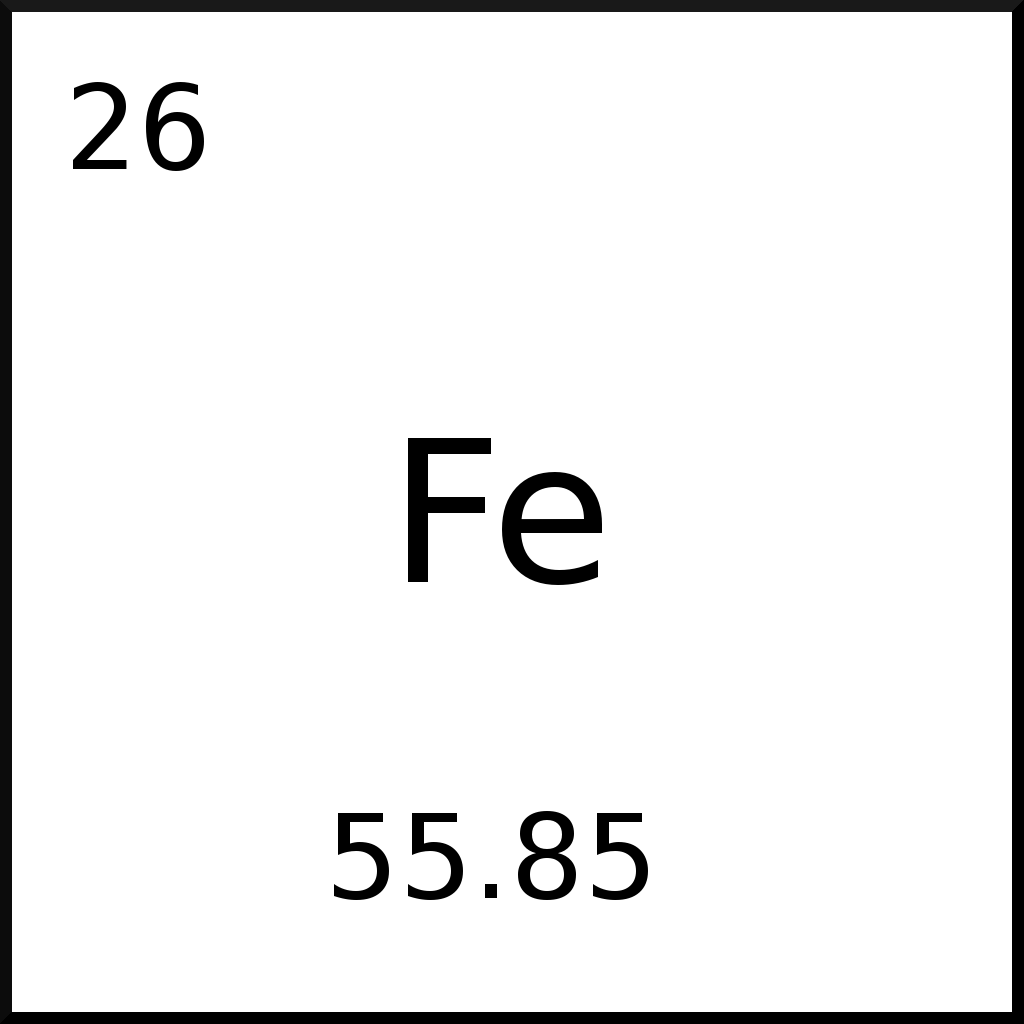
\includegraphics[width=2cm]{col11305.imgs/m38745_CG10C3_004.png} % m38745;CG10C3\_004.png;;;6.0;8.5;
      \vspace{2pt}
    \vspace{.1in}
    \end{center}
 \end{figure}       
      \par 
	\end{note}
	\end{minipage}
	\end{tabular}
	\par
      \label{m38745*id256193}You will notice in the example of iron that the atomic mass number is more or less the same as its atomic mass. Generally, an atom that contains \textsl{n} nucleons (protons and neutrons), will have a mass approximately equal to $n$u. For example the mass of a $\mathrm{C}-12$ atom which has 6 protons, 6 neutrons and 6 electrons is 12u, where the protons and neutrons have about the same mass and the electron mass is negligible. \par \pagebreak
\label{m38745*eip-950}\vspace{.5cm} 
      \noindent
      \hspace*{-30pt}
\includegraphics[width=0.5in]{col11305.imgs/pspencil2.png}   \raisebox{25mm}{   
      \begin{mdframed}[linewidth=4, leftmargin=40, rightmargin=40]  
      \begin{exercise}
    \noindent\textbf{Exercise 3.1}\label{m38745*eip-686}
  \label{m38745*eip-509}Use standard notation to represent sodium and give the number of protons, neutrons and electrons in the element.
  \par 
\vspace{5pt}
\label{m38745*eip-600}\noindent\textbf{Solution to Exercise }
  \label{m38745*eip-374}\label{m38745*listfhsst!!!underscore!!!id431}\begin{enumerate}[noitemsep, label=\textbf{Step} \textbf{\arabic*}. ] 
            \leftskip=20pt\rightskip=\leftskip\item Sodium is given by $Na$\item Sodium has 11 protons, so we have: ${}_{11}Na$\item Sodium has 12 neutrons.\item $A=N+Z=12+11=23$\item In standard notation sodium is given by: $_{11}^{23}Na$. The number of protons is 11, the number of neutrons is 12 and the number of electrons is 11.\end{enumerate}
  \par 
    \end{exercise}
    \end{mdframed}
    } \vspace{-.5cm}
    \noindent
  \label{m38745*secfhsst!!!underscore!!!id332}
            \subsubsection{  The structure of the atom
      }
            \nopagebreak
      \label{m38745*id256225}\begin{enumerate}[noitemsep, label=\textbf{\arabic*}. ] 
            \label{m38745*uid15}\item Explain the meaning of each of the following terms:
\label{m38745*id256240}\begin{enumerate}[noitemsep, label=\textbf{\alph*}. ] 
            \label{m38745*uid16}\item nucleus
\label{m38745*uid17}\item electron
\label{m38745*uid18}\item atomic mass
\end{enumerate}
                \label{m38745*uid19}\item Complete the following table: (Note: You will see that the atomic masses on the Periodic Table are not \textsl{whole numbers}. This will be explained later. For now, you can round off to the nearest whole number.)
    % \textbf{m38745*id256298}\par
          \begin{table}[H]
    % \begin{table}[H]
    % \\ 'id2886115' '1'
        \begin{center}
      \label{m38745*id256298}
    \noindent
    \tabletail{%
        \hline
        \multicolumn{6}{|p{\mytableboxwidth}|}{\raggedleft \small \sl continued on next page}\\
        \hline
      }
      \tablelasttail{}
      \begin{xtabular}[t]{|l|l|l|l|l|l|}\hline
        \textbf{Element} &
        \textbf{Atomic mass} &
        \textbf{Atomic number} &
        \textbf{Number of protons} &
        \textbf{Number of electrons} &
        \textbf{Number of neutrons}% make-rowspan-placeholders
     \tabularnewline\cline{1-1}\cline{2-2}\cline{3-3}\cline{4-4}\cline{5-5}\cline{6-6}
      %--------------------------------------------------------------------
        $Mg$ &
        24 &
        12 &
         &
         &
        % make-rowspan-placeholders
     \tabularnewline\cline{1-1}\cline{2-2}\cline{3-3}\cline{4-4}\cline{5-5}\cline{6-6}
      %--------------------------------------------------------------------
        $\mathrm{O}$ &
         &
         &
        8 &
         &
        % make-rowspan-placeholders
     \tabularnewline\cline{1-1}\cline{2-2}\cline{3-3}\cline{4-4}\cline{5-5}\cline{6-6}
      %--------------------------------------------------------------------
         &
         &
        17 &
         &
         &
        % make-rowspan-placeholders
     \tabularnewline\cline{1-1}\cline{2-2}\cline{3-3}\cline{4-4}\cline{5-5}\cline{6-6}
      %--------------------------------------------------------------------
        $Ni$ &
         &
         &
         &
        28 &
        % make-rowspan-placeholders
     \tabularnewline\cline{1-1}\cline{2-2}\cline{3-3}\cline{4-4}\cline{5-5}\cline{6-6}
      %--------------------------------------------------------------------
         &
        40 &
         &
         &
         &
        20% make-rowspan-placeholders
     \tabularnewline\cline{1-1}\cline{2-2}\cline{3-3}\cline{4-4}\cline{5-5}\cline{6-6}
      %--------------------------------------------------------------------
        $Zn$ &
         &
         &
         &
         &
        % make-rowspan-placeholders
     \tabularnewline\cline{1-1}\cline{2-2}\cline{3-3}\cline{4-4}\cline{5-5}\cline{6-6}
      %--------------------------------------------------------------------
         &
         &
         &
         &
         &
        0% make-rowspan-placeholders
     \tabularnewline\cline{1-1}\cline{2-2}\cline{3-3}\cline{4-4}\cline{5-5}\cline{6-6}
      %--------------------------------------------------------------------
        $\mathrm{C}$ &
        12 &
         &
         &
        6 &
        % make-rowspan-placeholders
     \tabularnewline\cline{1-1}\cline{2-2}\cline{3-3}\cline{4-4}\cline{5-5}\cline{6-6}
      %--------------------------------------------------------------------
    \end{xtabular}
      \end{center}
    \begin{center}{\small\bfseries Table 3.4}\end{center}
    \begin{caption}{\small\bfseries Table 3.4}\end{caption}
\end{table}
    \par
          \label{m38745*uid20}\item Use standard notation to represent the following elements:
\label{m38745*id256772}\begin{enumerate}[noitemsep, label=\textbf{\alph*}. ] 
            \label{m38745*uid21}\item potassium
\label{m38745*uid22}\item copper
\label{m38745*uid23}\item chlorine
\end{enumerate}
                \label{m38745*uid24}\item 
For the element $_{17}^{35}Cl$, give the number of ...
\label{m38745*id256843}\begin{enumerate}[noitemsep, label=\textbf{\alph*}. ] 
            \label{m38745*uid25}\item protons
\label{m38745*uid26}\item neutrons
\label{m38745*uid27}\item electrons
\end{enumerate}
... in the atom.\newline
\label{m38745*uid28}\item Which of the following atoms has 7 electrons?
\label{m38745*id256898}\begin{enumerate}[noitemsep, label=\textbf{\alph*}. ] 
            \label{m38745*uid29}\item $_{2}^{5}He$
\label{m38745*uid30}\item $_{6}^{13}\mathrm{C}$
\label{m38745*uid31}\item $_{3}^{7}Li$
\label{m38745*uid32}\item $_{7}^{15}\mathrm{N}$
\end{enumerate}
                \label{m38745*uid33}\item 
In each of the following cases, give the number or the element symbol represented by 'X'.
\label{m38745*id257023}\begin{enumerate}[noitemsep, label=\textbf{\alph*}. ] 
            \label{m38745*uid34}\item $_{18}^{40}\mathrm{X}$
\label{m38745*uid35}\item $_{20}^{x}\mathrm{Ca}$
\label{m38745*uid36}\item $_{x}^{31}\mathrm{P}$
\end{enumerate}
                \label{m38745*uid37}\item 
Complete the following table:
    % \textbf{m38745*id257121}\par
          \begin{table}[H]
    % \begin{table}[H]
    % \\ 'id2886554' '1'
        \begin{center}
      \label{m38745*id257121}
    \noindent
    \tabletail{%
        \hline
        \multicolumn{4}{|p{\mytableboxwidth}|}{\raggedleft \small \sl continued on next page}\\
        \hline
      }
      \tablelasttail{}
      \begin{xtabular}[t]{|l|l|l|l|}\hline
         &
        \textbf{A} &
        \textbf{Z} &
        \textbf{N}% make-rowspan-placeholders
     \tabularnewline\cline{1-1}\cline{2-2}\cline{3-3}\cline{4-4}
      %--------------------------------------------------------------------
        $_{92}^{235}\mathrm{U}$ &
         &
         &
        % make-rowspan-placeholders
     \tabularnewline\cline{1-1}\cline{2-2}\cline{3-3}\cline{4-4}
      %--------------------------------------------------------------------
        $_{92}^{238}\mathrm{U}$ &
         &
         &
        % make-rowspan-placeholders
     \tabularnewline\cline{1-1}\cline{2-2}\cline{3-3}\cline{4-4}
      %--------------------------------------------------------------------
    \end{xtabular}
      \end{center}
    \begin{center}{\small\bfseries Table 3.5}\end{center}
    \begin{caption}{\small\bfseries Table 3.5}\end{caption}
\end{table}
    \par
In these two different forms of Uranium...
\label{m38745*id257277}\begin{enumerate}[noitemsep, label=\textbf{\alph*}. ] 
            \label{m38745*uid38}\item What is the \textsl{same}?
\label{m38745*uid39}\item What is \textsl{different}?
\end{enumerate}
Uranium can occur in different forms, called \textsl{isotopes}. You will learn more about isotopes in "Isotopes".\newline
\end{enumerate}
  \label{m38745**end}
\par \raisebox{-5 pt}{
\includegraphics[width=0.5cm]{col11305.imgs/summary_www.png}} Find the answers with the shortcodes:
 \par \begin{tabular}[h]{cccccc}
 (1.) ll0  &  (2.) ll8  &  (3.) ll9  &  (4.) llX  &  (5.) llk  &  (6.) llK  &  (7.) llB  & \end{tabular}
         \section{ Isotopes}
    \nopagebreak
            \label{m38753} $ \hspace{-5pt}\begin{array}{cccccccccccc}   
\includegraphics[width=0.75cm]{col11305.imgs/summary_fullmarks.png} &   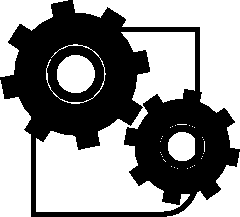
\includegraphics[width=0.75cm]{col11305.imgs/summary_simulation.png} &   \end{array} $ \hspace{2 pt}\raisebox{-5 pt}{} {(section shortcode: P10022 )} \par 
    \label{m38753*cid6}
            \subsection{ Isotopes}
            \nopagebreak
            \label{m38753*uid40}
            \subsubsection{ What is an isotope?}
            \nopagebreak
            \label{m38753*id257359}The chemical properties of an element depend on the number of protons and electrons inside the atom. So if a neutron or two is added or removed from the nucleus, then the chemical properties will not change. This means that such an atom would remain in the same place in the Periodic Table. For example, no matter how many neutrons we add or subtract from a nucleus with 6 protons, that element will \textbf{always} be called carbon and have the
element symbol $\mathrm{C}$ (see the Table of Elements). Atoms which have the same number of protons, but a different number of neutrons, are called \textbf{isotopes}.\par 
\label{m38753*fhsst!!!underscore!!!id386}\begin{definition}
	  \begin{tabular*}{15 cm}{m{15 mm}m{}}
	\hspace*{-50pt}  
\includegraphics[width=0.5in]{col11305.imgs/psflag2.png}   & \Definition{   \label{id2417667}\textbf{ Isotope }} { \label{m38753*meaningfhsst!!!underscore!!!id386}
        \label{m38753*id257386}The \textbf{isotope} of a particular element is made up of atoms which have the same number of protons as the atoms in the original element, but a different number of neutrons.  \par 
         } 
      \end{tabular*}
      \end{definition}
        \label{m38753*id257405}The different isotopes of an element have the same atomic
number $Z$ but different mass numbers $A$ because they have a different
number of neutrons $N$. The chemical properties of the different
isotopes of an element are the same, but they might vary in how stable their nucleus is. Note that we can also write elements as $\mathrm{X\; -\; A}$ where the X is the element symbol and the A is the atomic mass of that element. For example, $\mathrm{C-}12$ has an atomic mass of 12 and $\mathrm{Cl-}35$ has an atomic mass of 35 u, while $\mathrm{Cl-}37$ has an atomic mass of 37 u.\par 
\label{m38753*notfhsst!!!underscore!!!id393}
\begin{tabular}{cc}
	\hspace*{-50pt}\raisebox{-8 mm}{\hspace{-0.2in}
\includegraphics[width=0.75in]{col11305.imgs/psfact2.png} } & 
	\begin{minipage}{0.85\textwidth}
	\begin{note}
      {note: }
        \label{m38753*id257445}In Greek, ``same place'' reads as
$\stackrel{`}{\iota }\sigma o\varsigma $$\tau \stackrel{`}{o}\pi o\varsigma $\hspace{1ex}
(isos topos). This is why atoms which have the same number of protons, but
different numbers of neutrons, are called \textsl{isotopes}. They are in the same place on the Periodic Table!\par 
	\end{note}
	\end{minipage}
	\end{tabular}
	\par
\label{m38753*id248557}It is important to realise that the atomic mass of isotopes of the same element will be different because they have a different number of nucleons. Chlorine, for example, has two common isotopes which are chlorine-35 and chlorine-37. Chlorine-35 has an atomic mass of 35 u, while chlorine-37 has an atomic mass of 37 u. In the world around us, both of these isotopes occur naturally. It doesn't make sense to say that the element chlorine has an atomic mass of 35 u, or that it has an atomic mass of 37 u. Neither of these are absolutely true since the mass varies depending on the form in which the element occurs. We need to look at how much more common one is than the other in order to calculate the \textbf{relative atomic mass} for the element chlorine. This is the number that you find on the Periodic Table.\par 
\label{m38753*eip-8228}
\begin{tabular}{cc}
	\hspace*{-50pt}\raisebox{-8 mm}{\hspace{-0.2in}
\includegraphics[width=0.75in]{col11305.imgs/psfact2.png} } & 
	\begin{minipage}{0.85\textwidth}
	\begin{note}
      {note: }\label{m38753*id9742331}The relative atomic mass of some elements depends on where on Earth the element is found. This is because the isotopes can be found in varying ratios depending on certain factors such as geological composition, etc. The International Union of Pure and Applied Chemistry (IUPAC) has decided to give the relative atomic mass of some elements as a range to better represent the varying isotope ratios on the Earth. For the calculations that you will do at high school, it is enough to simply use one number without worrying about these ranges.\par 
	\end{note}
	\end{minipage}
	\end{tabular}
	\par \pagebreak
      \label{m38753*secfhsst!!!underscore!!!id2602}\vspace{.5cm} 
      \noindent
      \hspace*{-30pt}
\includegraphics[width=0.5in]{col11305.imgs/pspencil2.png}   \raisebox{25mm}{   
      \begin{mdframed}[linewidth=4, leftmargin=40, rightmargin=40]  
      \begin{exercise}
    \noindent\textbf{Exercise 3.2:  The relative atomic mass of an isotopic element }
        \label{m38753*probfhsst!!!underscore!!!id6203}
        \label{m38753*id2586016}The element chlorine has two isotopes, chlorine-35 and chlorine-37. The abundance of these isotopes when they occur naturally is 75\% chlorine-35 and 25\% chlorine-37. Calculate the \textsl{average} relative atomic mass for chlorine.
 \par 
        \vspace{5pt}
        \label{m38753*solfhsst!!!underscore!!!id6207}\noindent\textbf{Solution to Exercise } \label{m38753*listfhsst!!!underscore!!!id6107}\begin{enumerate}[noitemsep, label=\textbf{Step} \textbf{\arabic*}. ] 
            \leftskip=20pt\rightskip=\leftskip\item  
        \label{m38753*id2582637}Contribution of $\mathrm{Cl-}35=\left(\frac{75}{100}\ensuremath{\times}35\right)=26,25\phantom{\rule{2pt}{0ex}}\mathrm{u}$
 \par 
        \item  
        \label{m38753*id2528657}Contribution of $\mathrm{Cl-}37=\left(\frac{25}{100}\ensuremath{\times}37\right)=9,25\phantom{\rule{2pt}{0ex}}\mathrm{u}$\par 
        \item  
        \label{m38753*id2586730}$\mathrm{Relative\; atomic\; mass\; of\; chlorine}=26,25\phantom{\rule{2pt}{0ex}}\mathrm{u}+9,25\phantom{\rule{2pt}{0ex}}\mathrm{u}=35,5\phantom{\rule{2pt}{0ex}}\mathrm{u}$\par 
        \label{m38753*id2586714}If you look on the periodic table, the average relative atomic mass for chlorine is $35,5\phantom{\rule{2pt}{0ex}}\mathrm{u}$. You will notice that for many elements, the relative atomic mass that is shown is not a whole number. You should now understand that this number is the \textsl{average} relative atomic mass for those elements that have naturally occurring isotopes.\par 
\end{enumerate}
    \end{exercise}
    \end{mdframed}
    }
    \noindent
This simulation allows you to see how isotopes and relative atomic mass are inter related.
    \setcounter{subfigure}{0}
	\begin{figure}[H] % horizontal\label{m38806*transverse-waves}
    \textnormal{Phet simulation for Isotopes}\vspace{.1in} \nopagebreak
  \label{m38806*phet!!!underscore!!!sim}\label{m38806*phet-simulation}
            \raisebox{-5 pt}{ 
\includegraphics[width=0.5cm]{col11305.imgs/summary_www.png}} { (Simulation:  lbT )}
      \vspace{2pt}
    \vspace{.1in}
 \end{figure}           \par \label{m38753*secfhsst!!!underscore!!!id6128}
            \subsubsection{  Isotopes }
            \nopagebreak
        \label{m38753*id25862299}\begin{enumerate}[noitemsep, label=\textbf{\arabic*}. ] 
            \label{m38753*uid619}\item Complete the table below:
    % \textbf{m38753*id25871115}\par
          \begin{table}[H]
    % \begin{table}[H]
    % \\ 'id2887415' '1'
        \begin{center}
      \label{m38753*id25871115}
    \noindent
    \tabletail{%
        \hline
        \multicolumn{6}{|p{\mytableboxwidth}|}{\raggedleft \small \sl continued on next page}\\
        \hline
      }
      \tablelasttail{}
      \begin{xtabular}[t]{|l|l|l|l|l|l|}\hline
        \textbf{Isotope} &
        \textbf{Z} &
        \textbf{A} &
        \textbf{Protons} &
        \textbf{Neutrons} &
        \textbf{Electrons}% make-rowspan-placeholders
     \tabularnewline\cline{1-1}\cline{2-2}\cline{3-3}\cline{4-4}\cline{5-5}\cline{6-6}
      %--------------------------------------------------------------------
        Carbon-12 &
         &
         &
         &
         &
        % make-rowspan-placeholders
     \tabularnewline\cline{1-1}\cline{2-2}\cline{3-3}\cline{4-4}\cline{5-5}\cline{6-6}
      %--------------------------------------------------------------------
        Carbon-14 &
         &
         &
         &
         &
        % make-rowspan-placeholders
     \tabularnewline\cline{1-1}\cline{2-2}\cline{3-3}\cline{4-4}\cline{5-5}\cline{6-6}
      %--------------------------------------------------------------------
        Chlorine-35 &
         &
         &
         &
         &
        % make-rowspan-placeholders
     \tabularnewline\cline{1-1}\cline{2-2}\cline{3-3}\cline{4-4}\cline{5-5}\cline{6-6}
      %--------------------------------------------------------------------
        Chlorine-37 &
         &
         &
         &
         &
        % make-rowspan-placeholders
     \tabularnewline\cline{1-1}\cline{2-2}\cline{3-3}\cline{4-4}\cline{5-5}\cline{6-6}
      %--------------------------------------------------------------------
    \end{xtabular}
      \end{center}
    \begin{center}{\small\bfseries Table 3.6}\end{center}
    \begin{caption}{\small\bfseries Table 3.6}\end{caption}
\end{table}
    \par
          \label{m38753*uid7170}\item If a sample contains 90\% carbon-12 and 10\% carbon-14, calculate the relative atomic mass of an atom in that sample.
\hspace{1ex}        \label{m38753*uid7100}\item If a sample contains 22,5\% Cl-37 and 77,5\% Cl-35, calculate the relative atomic mass of an atom in that sample.\hspace{1ex}        
\end{enumerate}
      \label{m38753*id255886}Standard notation shows the chemical symbol, the atomic mass number
and the atomic number of an element as follows:\par 
      \label{m38753*id255890}
    \setcounter{subfigure}{0}
	\begin{figure}[H] % horizontal\label{m38753*id255893}
    \begin{center}
    \label{m38753*id255893!!!underscore!!!media}\label{m38753*id255893!!!underscore!!!printimage}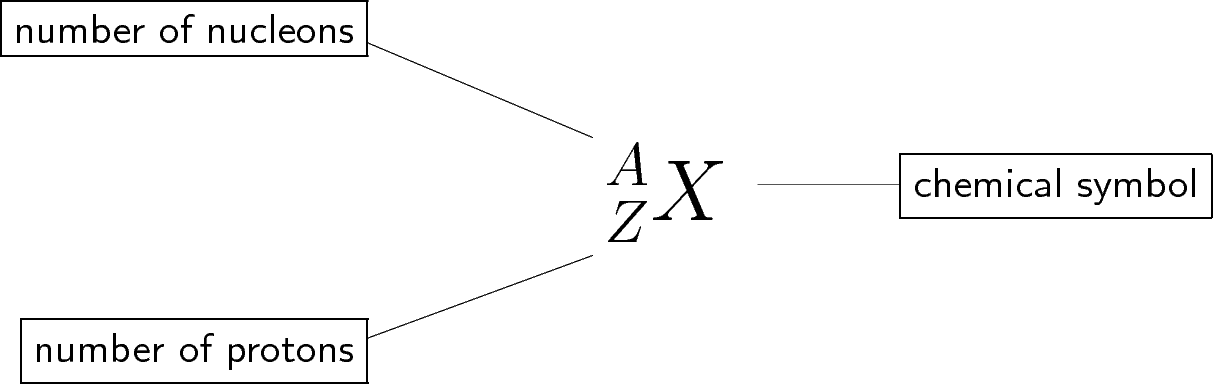
\includegraphics{col11305.imgs/m38753_atom_sym.png} % m38753;atom\_sym.png;;;6.0;8.5;
      \vspace{2pt}
    \vspace{.1in}
    \end{center}
 \end{figure}       
      \par 
      \label{m38753*eip-741}
\begin{tabular}{cc}
	\hspace*{-50pt}\raisebox{-8 mm}{\hspace{-0.2in}
\includegraphics[width=0.75in]{col11305.imgs/psfact2.png} } & 
	\begin{minipage}{0.85\textwidth}
	\begin{note}
      {note: }A nuclide is a distinct kind of atom or nucleus characterized by the number of protons and neutrons in the atom. To be absolutely correct, when we represent atoms like we do here, then we should call them nuclides. 
	\end{note}
	\end{minipage}
	\end{tabular}
	\par
      \label{m38753*id255900}For example, the iron nucleus which has 26 protons and 30 neutrons, is
denoted as:\par 
      \label{m38753*id255904}\nopagebreak\noindent{}
        
    \begin{equation}
    _{26}^{56}\mathrm{Fe}\phantom{\rule{4pt}{0ex}}\tag{3.1}
      \end{equation}
      \label{m38753*id255929}where the atomic number is $Z=26$\hspace{1ex} and the mass number $A=56$.
The number of neutrons is simply the difference $N=A-Z$.\par 
        \label{m38753*id257512}The following worked examples will help you to understand the concept of an isotope better.\par \pagebreak
\label{m38753*secfhsst!!!underscore!!!id400}\vspace{.5cm} 
      \noindent
      \hspace*{-30pt}
\includegraphics[width=0.5in]{col11305.imgs/pspencil2.png}   \raisebox{25mm}{   
      \begin{mdframed}[linewidth=4, leftmargin=40, rightmargin=40]  
      \begin{exercise}
    \noindent\textbf{Exercise 3.3:  Isotopes  }
        \label{m38753*probfhsst!!!underscore!!!id401}
        \label{m38753*id257529}For the element $_{92}^{234}\mathrm{U}$ (uranium), use standard notation to describe:\par 
        \label{m38753*id257558}\begin{enumerate}[noitemsep, label=\textbf{\arabic*}. ] 
            \leftskip=20pt\rightskip=\leftskip\label{m38753*uid41}\item the isotope with 2 fewer neutrons
\label{m38753*uid42}\item the isotope with 4 more neutrons
\end{enumerate}
        \vspace{5pt}
        \label{m38753*solfhsst!!!underscore!!!id411}\noindent\textbf{Solution to Exercise } \label{m38753*listfhsst!!!underscore!!!id411}\begin{enumerate}[noitemsep, label=\textbf{Step} \textbf{\arabic*}. ] 
            \leftskip=20pt\rightskip=\leftskip\item  
        \label{m38753*id257607}We know that isotopes of any element have the \textbf{same} number
of protons (same atomic number)
in each atom, which means that they have the same chemical symbol. However, they have a different number of neutrons, and therefore a different mass number.\par 
        \item  
        \label{m38753*id257640}Therefore, any isotope of uranium will have the symbol:\par 
        \label{m38753*id257644}\nopagebreak\noindent{}
          
    \begin{equation}
    \mathrm{U}\tag{3.2}
      \end{equation}
        \label{m38753*id257657}Also, since the number of protons in uranium isotopes is always the same, we can write
down the atomic number:\par 
        \label{m38753*id257664}\nopagebreak\noindent{}
          
    \begin{equation}
    {}_{92}\mathrm{U}\tag{3.3}
      \end{equation}
        \label{m38753*id257684}Now, if the isotope we want has 2 fewer neutrons than $_{92}^{234}\mathrm{U}$,
then we take the original mass number and subtract 2, which gives:\par 
        \label{m38753*id257713}\nopagebreak\noindent{}
          
    \begin{equation}
    _{92}^{232}\mathrm{U}\tag{3.4}
      \end{equation}
        \label{m38753*id257736}Following the steps above, we can write the isotope with 4 more neutrons as:\par 
        \label{m38753*id257740}\nopagebreak\noindent{}
          
    \begin{equation}
    _{92}^{238}\mathrm{U}\tag{3.5}
      \end{equation}
 \end{enumerate}
    \end{exercise}
    \end{mdframed}
    }
    \noindent
\par
            \label{m38753*secfhsst!!!underscore!!!id466}\vspace{.5cm} 
      \noindent
      \hspace*{-30pt}
\includegraphics[width=0.5in]{col11305.imgs/pspencil2.png}   \raisebox{25mm}{   
      \begin{mdframed}[linewidth=4, leftmargin=40, rightmargin=40]  
      \begin{exercise}
    \noindent\textbf{Exercise 3.4:  Isotopes }
        \label{m38753*probfhsst!!!underscore!!!id467}
        \label{m38753*id257776}Which of the following are isotopes of $_{20}^{40}\mathrm{Ca}$?\par 
        \label{m38753*id257802}\begin{itemize}[noitemsep]
            \leftskip=20pt\rightskip=\leftskip\label{m38753*uid43}\item 
            $_{19}^{40}\mathrm{K}$
          \label{m38753*uid44}\item 
            $_{20}^{42}\mathrm{Ca}$
          \label{m38753*uid45}\item 
            $_{18}^{40}\mathrm{Ar}$
          \end{itemize}
        \vspace{5pt}
        \label{m38753*solfhsst!!!underscore!!!id509}\noindent\textbf{Solution to Exercise } \label{m38753*listfhsst!!!underscore!!!id509}\begin{enumerate}[noitemsep, label=\textbf{Step} \textbf{\arabic*}. ] 
            \leftskip=20pt\rightskip=\leftskip\item  
        \label{m38753*id257917}We know that isotopes have the same atomic number but different mass numbers.\par 
        \item  
        \label{m38753*id257943}You need to look for the element that has the same atomic number but a different atomic mass number. The only element is $_{20}^{42}Ca$. What is different is that there are 2 more neutrons than in the original element.\par 
\end{enumerate}
    \end{exercise}
    \end{mdframed}
    }
    \noindent
\label{m38753*secfhsst!!!underscore!!!id517}\vspace{.5cm} 
      \noindent
      \hspace*{-30pt}
\includegraphics[width=0.5in]{col11305.imgs/pspencil2.png}   \raisebox{25mm}{   
      \begin{mdframed}[linewidth=4, leftmargin=40, rightmargin=40]  
      \begin{exercise}
    \noindent\textbf{Exercise 3.5:  Isotopes }
        \label{m38753*probfhsst!!!underscore!!!id518}
        \label{m38753*id257977}For the sulphur isotope $_{16}^{33}\mathrm{S}$, give the number of...\par 
        \label{m38753*id258000}\begin{enumerate}[noitemsep, label=\textbf{\alph*}. ] 
            \leftskip=20pt\rightskip=\leftskip\label{m38753*uid46}\item protons
\label{m38753*uid47}\item nucleons
\label{m38753*uid48}\item electrons
\label{m38753*uid49}\item neutrons
\end{enumerate}
        \vspace{5pt}
        \label{m38753*solfhsst!!!underscore!!!id532}\noindent\textbf{Solution to Exercise } \label{m38753*listfhsst!!!underscore!!!id532}\begin{enumerate}[noitemsep, label=\textbf{Step} \textbf{\arabic*}. ] 
            \leftskip=20pt\rightskip=\leftskip\item  
        \label{m38753*id258074}$Z=16$, therefore the number of protons is 16 (answer to (a)).
 \par 
        \item  
        \label{m38753*id258094}$A=33$, therefore the number of nucleons is 33 (answer to (b)).\par 
        \item  
        \label{m38753*id258102}The atom is neutral, and therefore the number of electrons is the same as the number of protons. The number of electrons is 16 (answer to (c)).\par 
        \item  
        \label{m38753*id258110}\nopagebreak\noindent{}
          
    \begin{equation}
    \begin{array}{c}\hfill N=A-Z=33-16=17\end{array}\tag{3.6}
      \end{equation}
        \label{m38753*id258151}The number of neutrons is 17 (answer to (d)).\par 
\end{enumerate}
    \end{exercise}
    \end{mdframed}
    }
    \noindent
% \label{m38753*secfhsst!!!underscore!!!id567}
% \par \raisebox{-5 pt}{
\includegraphics[width=0.5cm]{col11305.imgs/summary_www.png}} Find the answers with the shortcodes:
%  \par \begin{tabular}[h]{cccccc}
%  (1.) llj  &  (2.) llb  &  (3.) llT  & \end{tabular}
            \subsubsection{  Isotopes }
            \nopagebreak
        \label{m38753*id258162}\begin{enumerate}[noitemsep, label=\textbf{\arabic*}. ] 
            \label{m38753*uid50}\item Atom A has 5 protons and 5 neutrons, and atom B has 6 protons and 5 neutrons. These atoms are...
\label{m38753*id258178}\begin{enumerate}[noitemsep, label=\textbf{\alph*}. ] 
            \label{m38753*uid51}\item allotropes
\label{m38753*uid52}\item isotopes
\label{m38753*uid53}\item isomers
\label{m38753*uid54}\item atoms of different elements
\end{enumerate}
                \label{m38753*uid55}\item For the sulphur isotopes, $_{16}^{32}\mathrm{S}$ and $_{16}^{34}\mathrm{S}$, give the number of...
\label{m38753*id258277}\begin{enumerate}[noitemsep, label=\textbf{\alph*}. ] 
            \label{m38753*uid56}\item protons
\label{m38753*uid57}\item nucleons
\label{m38753*uid58}\item electrons
\label{m38753*uid59}\item neutrons
\end{enumerate}
                \label{m38753*uid60}\item Which of the following are isotopes of $_{17}^{35}\mathrm{Cl}$?
\label{m38753*id258355}\begin{enumerate}[noitemsep, label=\textbf{\alph*}. ] 
            \label{m38753*uid61}\item $_{35}^{17}\mathrm{Cl}$
\label{m38753*uid62}\item $_{17}^{35}\mathrm{Cl}$
\label{m38753*uid63}\item $_{17}^{37}\mathrm{Cl}$
\end{enumerate}
                \label{m38753*uid64}\item Which of the following are isotopes of $\mathrm{U-}235$? (X represents an element symbol)
\label{m38753*id258452}\begin{enumerate}[noitemsep, label=\textbf{\alph*}. ] 
            \label{m38753*uid65}\item $_{92}^{238}\mathrm{X}$
\label{m38753*uid66}\item $_{90}^{238}\mathrm{X}$
\label{m38753*uid67}\item $_{92}^{235}\mathrm{X}$
\end{enumerate}
                \end{enumerate}
      \label{m38753*uid68}
\par \raisebox{-5 pt}{
\includegraphics[width=0.5cm]{col11305.imgs/summary_www.png}} Find the answers with the shortcodes:
 \par \begin{tabular}[h]{cccccc}
 (1.) ll4  &  (2.) llZ  &  (3.) llW  &  (4.) llD  & \end{tabular}
            \subsubsection{ Relative atomic mass}
            \nopagebreak
            \label{m38753*id258557}It is important to realise that the atomic mass of isotopes of the same element will be different because they have a different number of nucleons. Chlorine, for example, has two common isotopes which are chlorine-35 and chlorine-37. Chlorine-35 has an atomic mass of 35 u, while chlorine-37 has an atomic mass of 37 u. In the world around us, both of these isotopes occur naturally. It doesn't make sense to say that the element chlorine has an atomic mass of 35 u, or that it has an atomic mass of 37 u. Neither of these are absolutely true since the mass varies depending on the form in which the element occurs. We need to look at how much more common one is than the other in order to calculate the \textbf{relative atomic mass} for the element chlorine. This is the number that you find on the Periodic Table.\par 
\label{m38753*eip-828}
\begin{tabular}{cc}
	\hspace*{-50pt}\raisebox{-8 mm}{\hspace{-0.2in}
\includegraphics[width=0.75in]{col11305.imgs/psfact2.png} } & 
	\begin{minipage}{0.85\textwidth}
	\begin{note}
      {note: }\label{m38753*id97421}The relative atomic mass of some elements depends on where on Earth the element is found. This is because the isotopes can be found in varying ratios depending on certain factors such as geological composition, etc. The International Union of Pure and Applied Chemistry (IUPAC) has decided to give the relative atomic mass of some elements as a range to better represent the varying isotope ratios on the Earth. For the calculations that you will do at high school, it is enough to simply use one number without worrying about these ranges.\par 
	\end{note}
	\end{minipage}
	\end{tabular}
	\par
      \label{m38753*secfhsst!!!underscore!!!id602}\vspace{.5cm} 
      \noindent
      \hspace*{-30pt}
\includegraphics[width=0.5in]{col11305.imgs/pspencil2.png}   \raisebox{25mm}{   
      \begin{mdframed}[linewidth=4, leftmargin=40, rightmargin=40]  
      \begin{exercise}
    \noindent\textbf{Exercise 3.6:  The relative atomic mass of an isotopic element }
        \label{m38753*probfhsst!!!underscore!!!id603}
        \label{m38753*id258606}The element chlorine has two isotopes, chlorine-35 and chlorine-37. The abundance of these isotopes when they occur naturally is 75\% chlorine-35 and 25\% chlorine-37. Calculate the \textsl{average} relative atomic mass for chlorine.
 \par 
        \vspace{5pt}
        \label{m38753*solfhsst!!!underscore!!!id607}\noindent\textbf{Solution to Exercise } \label{m38753*listfhsst!!!underscore!!!id607}\begin{enumerate}[noitemsep, label=\textbf{Step} \textbf{\arabic*}. ] 
            \leftskip=20pt\rightskip=\leftskip\item  
        \label{m38753*id258637}Contribution of $\mathrm{Cl-}35=\left(\frac{75}{100}\ensuremath{\times}35\right)=26,25\phantom{\rule{2pt}{0ex}}\mathrm{u}$
 \par 
        \item  
        \label{m38753*id258657}Contribution of $\mathrm{Cl-}37=\left(\frac{25}{100}\ensuremath{\times}37\right)=9,25\phantom{\rule{2pt}{0ex}}\mathrm{u}$\par 
        \item  
        \label{m38753*id258670}$\mathrm{Relative\; atomic\; mass\; of\; chlorine}=26,25\phantom{\rule{2pt}{0ex}}\mathrm{u}+9,25\phantom{\rule{2pt}{0ex}}\mathrm{u}=35,5\phantom{\rule{2pt}{0ex}}\mathrm{u}$\par 
        \label{m38753*id258674}If you look on the periodic table, the average relative atomic mass for chlorine is $35,5\phantom{\rule{2pt}{0ex}}\mathrm{u}$. You will notice that for many elements, the relative atomic mass that is shown is not a whole number. You should now understand that this number is the \textsl{average} relative atomic mass for those elements that have naturally occurring isotopes.\par 
\end{enumerate}
    \end{exercise}
    \end{mdframed}
    }
    \noindent
        \par \label{m38753*secfhsst!!!underscore!!!id618}
            \subsubsection{  Isotopes }
            \nopagebreak
        \label{m38753*id258699}\begin{enumerate}[noitemsep, label=\textbf{\arabic*}. ] 
            \label{m38753*uid69}\item Complete the table below:
    % \textbf{m38753*id258715}\par
          \begin{table}[H]
    % \begin{table}[H]
    % \\ 'id2889162' '1'
        \begin{center}
      \label{m38753*id258715}
    \noindent
    \tabletail{%
        \hline
        \multicolumn{6}{|p{\mytableboxwidth}|}{\raggedleft \small \sl continued on next page}\\
        \hline
      }
      \tablelasttail{}
      \begin{xtabular}[t]{|l|l|l|l|l|l|}\hline
        \textbf{Isotope} &
        \textbf{Z} &
        \textbf{A} &
        \textbf{Protons} &
        \textbf{Neutrons} &
        \textbf{Electrons}% make-rowspan-placeholders
     \tabularnewline\cline{1-1}\cline{2-2}\cline{3-3}\cline{4-4}\cline{5-5}\cline{6-6}
      %--------------------------------------------------------------------
        Carbon-12 &
         &
         &
         &
         &
        % make-rowspan-placeholders
     \tabularnewline\cline{1-1}\cline{2-2}\cline{3-3}\cline{4-4}\cline{5-5}\cline{6-6}
      %--------------------------------------------------------------------
        Carbon-14 &
         &
         &
         &
         &
        % make-rowspan-placeholders
     \tabularnewline\cline{1-1}\cline{2-2}\cline{3-3}\cline{4-4}\cline{5-5}\cline{6-6}
      %--------------------------------------------------------------------
        Chlorine-35 &
         &
         &
         &
         &
        % make-rowspan-placeholders
     \tabularnewline\cline{1-1}\cline{2-2}\cline{3-3}\cline{4-4}\cline{5-5}\cline{6-6}
      %--------------------------------------------------------------------
        Chlorine-37 &
         &
         &
         &
         &
        % make-rowspan-placeholders
     \tabularnewline\cline{1-1}\cline{2-2}\cline{3-3}\cline{4-4}\cline{5-5}\cline{6-6}
      %--------------------------------------------------------------------
    \end{xtabular}
      \end{center}
    \begin{center}{\small\bfseries Table 3.7}\end{center}
    \begin{caption}{\small\bfseries Table 3.7}\end{caption}
\end{table}
    \par
          \label{m38753*uid70}\item If a sample contains 90\% carbon-12 and 10\% carbon-14, calculate the relative atomic mass of an atom in that sample.
\hspace{1ex}        \label{m38753*uid71}\item If a sample contains 22,5\% Cl-37 and 77,5\% Cl-35, calculate the relative atomic mass of an atom in that sample.\hspace{1ex}        
\end{enumerate}
  \label{m38753**end}
\par \raisebox{-5 pt}{
\includegraphics[width=0.5cm]{col11305.imgs/summary_www.png}} Find the answers with the shortcodes:
 \par \begin{tabular}[h]{cccccc}
 (1.) llj  &  (2.) llb  &  (3.) llT  & \end{tabular}
         \section{ Electronic structure}
    \nopagebreak
            \label{m38741} $ \hspace{-5pt}\begin{array}{cccccccccccc}   
\includegraphics[width=0.75cm]{col11305.imgs/summary_fullmarks.png} &   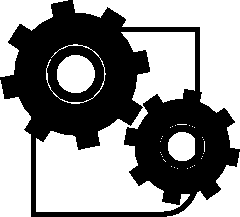
\includegraphics[width=0.75cm]{col11305.imgs/summary_simulation.png} &   
\includegraphics[width=0.75cm]{col11305.imgs/summary_video.png} &   
\includegraphics[width=0.75cm]{col11305.imgs/summary_presentation.png} &   \end{array} $ \hspace{2 pt}\raisebox{-5 pt}{} {(section shortcode: P10023 )} \par 
    \label{m38741*cid7}
            \subsection{ Electron configuration}
            \nopagebreak
      \label{m38741*uid79}
            \subsubsection{ The energy of electrons}
            \nopagebreak
        \label{m38741*id259210}You will remember from our earlier discussions that an atom is made up of a central nucleus, which contains protons and neutrons and that this nucleus is surrounded by electrons. Although these electrons all have the same charge and the same mass, each electron in an atom has a different amount of \textsl{energy}. Electrons that have the \textsl{lowest} energy are found closest to the nucleus where the attractive force of the positively charged nucleus is the greatest. Those electrons that have \textsl{higher} energy, and which are able to overcome the attractive force of the nucleus, are found further away.\par 
      \label{m38741*uid81}
            \subsubsection{ Electron configuration}
            \nopagebreak
            \label{m38741*id9722401}We will start with a very simple view of the arrangement or configuration of electrons around an atom. This view simply states that electrons are arranged in energy levels (or shells) around the nucleus of an atom. These energy levels are numbered 1, 2, 3, etc. Electrons that are in the first energy level (energy level 1) are closest to the nucleus and will have the lowest energy. Electrons further away from the nucleus will have a higher energy. \par 
\label{m38741*id259357}In the following examples, the energy levels are shown as concentric circles around the central nucleus. The important thing to know for these diagrams is that the first energy level can hold 2 electrons, the second energy level can hold 8 electrons and the third energy level can hold 8 electrons.\par 
        \label{m38741*id259361}\begin{enumerate}[noitemsep, label=\textbf{\arabic*}. ] 
            \label{m38741*uid86}\item \textbf{Lithium}
Lithium (Li) has an atomic number of 3, meaning that in a neutral atom, the number of electrons will also be 3. The first two electrons are found in the first energy level, while the third electron is found in the second energy level (Figure~3.9).
    \setcounter{subfigure}{0}
	\begin{figure}[H] % horizontal\label{m38741*uid87}
    \begin{center}
    \label{m38741*uid87!!!underscore!!!media}\label{m38741*uid87!!!underscore!!!printimage}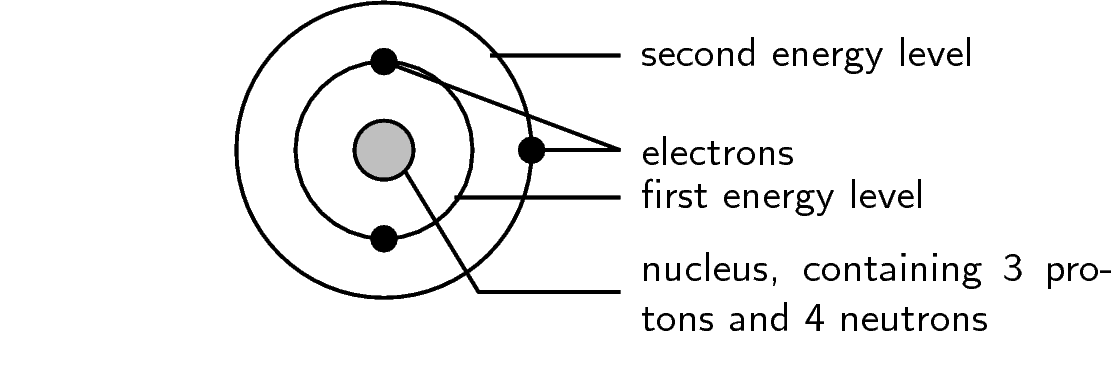
\includegraphics[width=300px]{col11305.imgs/m38741_CG10C3_005.png} % m38741;CG10C3\_005.png;;;6.0;8.5;
      \vspace{2pt}
    \vspace{\rubberspace}\par \begin{cnxcaption}
	  \small \textbf{Figure 3.9: }The arrangement of electrons in a lithium atom.
	\end{cnxcaption}
    \vspace{.1in}
    \end{center}
 \end{figure}       \label{m38741*uid88}\item \textbf{Fluorine}
Fluorine ($\mathrm{F}$) has an atomic number of 9, meaning that a neutral atom also has 9 electrons. The first 2 electrons are found in the first energy level, while the other 7 are found in the second energy level (Figure~3.10).
    \setcounter{subfigure}{0}
	\begin{figure}[H] % horizontal\label{m38741*uid89}
    \begin{center}
    \label{m38741*uid89!!!underscore!!!media}\label{m38741*uid89!!!underscore!!!printimage}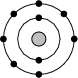
\includegraphics[width=2cm]{col11305.imgs/m38741_CG10C3_006.png} % m38741;CG10C3\_006.png;;;6.0;8.5;
      \vspace{2pt}
    \vspace{\rubberspace}\par \begin{cnxcaption}
	  \small \textbf{Figure 3.10: }The arrangement of electrons in a fluorine atom.
	\end{cnxcaption}
    \vspace{.1in}
    \end{center}
 \end{figure}       \label{m38741*uid90}\item \textbf{Argon}
Argon has an atomic number of 18, meaning that a neutral atom also has 18 electrons. The first 2 electrons are found in the first energy level, the next 8 are found in the second energy level, and the last 8 are found in the third energy level (Figure~3.11).
    \setcounter{subfigure}{0}
	\begin{figure}[H] % horizontal\label{m38741*uid91}
    \begin{center}
    \label{m38741*uid91!!!underscore!!!media}\label{m38741*uid91!!!underscore!!!printimage}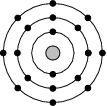
\includegraphics[width=2cm]{col11305.imgs/m38741_CG10C3_007.png} % m38741;CG10C3\_007.png;;;6.0;8.5;
      \vspace{2pt}
    \vspace{\rubberspace}\par \begin{cnxcaption}
	  \small \textbf{Figure 3.11: }The arrangement of electrons in an argon atom.
	\end{cnxcaption}
    \vspace{.1in}
    \end{center}
 \end{figure}       \end{enumerate}
\label{m38741*id259478}But the situation is slightly more complicated than this. Within each energy level, the electrons move in \textbf{orbitals}. An orbital defines the spaces or regions where electrons move.\par 
\label{m38741*fhsst!!!underscore!!!id687}\begin{definition}
	  \begin{tabular*}{15 cm}{m{15 mm}m{}}
	\hspace*{-50pt}  
\includegraphics[width=0.5in]{col11305.imgs/psflag2.png}   & \Definition{   \label{id2420554}\textbf{ Atomic orbital }} { \label{m38741*meaningfhsst!!!underscore!!!id687}
        \label{m38741*id259495}An atomic orbital is the region in which an electron may be found around a single atom.
 \par 
         } 
      \end{tabular*}
      \end{definition}
\label{m38741*id6732}
The first energy level contains only one 's' orbital, the second energy level contains one 's' orbital and three 'p' orbitals and the third energy level contains one 's' orbital and three 'p' orbitals (as well as 5 'd' orbitals). Within each energy level, the 's' orbital is at a lower energy than the 'p' orbitals. This arrangement is shown in Figure~3.12.\par 
    \setcounter{subfigure}{0}
	\begin{figure}[H] % horizontal\label{m38741*uid92}
    \begin{center}
    \rule[.1in]{\figurerulewidth}{.005in} \\
        \label{m38741*uid92!!!underscore!!!media}\label{m38741*uid92!!!underscore!!!printimage}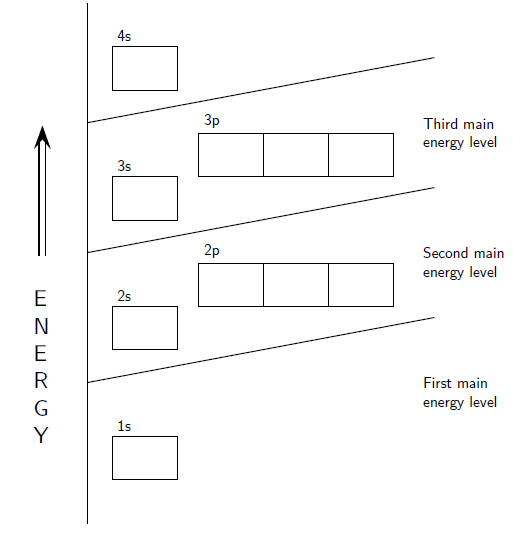
\includegraphics[height=300px]{col11305.imgs/m38741_CG10C3_008.png} % m38741;CG10C3\_008.png;;;6.0;8.5;
      \vspace{2pt}
    \vspace{\rubberspace}\par \begin{cnxcaption}
	  \small \textbf{Figure 3.12: }The positions of the first ten orbitals of an atom on an energy diagram. Note that each block is able to hold two electrons.
	\end{cnxcaption}
    \vspace{.1in}
    \rule[.1in]{\figurerulewidth}{.005in} \\
    \end{center}
 \end{figure}       
        \label{m38741*eip-752}This diagram also helps us when we are working out the electron configuration of an element. The electron configuration of an element is the arrangement of the electrons in the shells and subshells. There are a few guidelines for working out the electron configuration. These are:
\par \label{m38741*id259303}\begin{itemize}[noitemsep]
            \label{m38741*uid93}\item Each orbital can only hold \textbf{two electrons}. Electrons that occur together in an orbital are called an \textbf{electron pair}.
\label{m38741*uid94}\item An electron will always try to enter an orbital with the lowest possible energy.
\label{m38741*uid95}\item An electron will occupy an orbital on its own, rather than share an orbital with another electron. An electron would also rather occupy a lower energy orbital \textsl{with} another electron, before occupying a higher energy orbital. In other words, within one energy level, electrons will fill an 's' orbital before starting to fill 'p' orbitals.
\label{m38741*uid83}\item The s subshell can hold 2 electrons
\label{m38741*uid84}\item The p subshell can hold 6 electrons
\end{itemize}
        \label{m38741*eip-15}In the examples you will cover, you will mainly be filling the s and p subshells. Occasionally you may get an example that has the d subshell. The f subshell is more complex and is not covered at this level.
\par 
        \label{m38741*id259599}The way that electrons are arranged in an atom is called its \textbf{electron configuration}.\par 
\label{m38741*fhsst!!!underscore!!!id709}\begin{definition}
	  \begin{tabular*}{15 cm}{m{15 mm}m{}}
	\hspace*{-50pt}  
\includegraphics[width=0.5in]{col11305.imgs/psflag2.png}   & \Definition{   \label{id2420737}\textbf{ Electron configuration }} { \label{m38741*meaningfhsst!!!underscore!!!id709}
        \label{m38741*id259615}Electron configuration is the arrangement of electrons in an atom, molecule or other physical structure. \par 
         } 
      \end{tabular*}
      \end{definition}
        \label{m38741*id259628}An element's electron configuration can be represented using \textbf{Aufbau diagrams} or energy level diagrams. An Aufbau diagram uses arrows to represent electrons. You can use the following steps to help you to draw an Aufbau diagram:\par 
        \label{m38741*id259639}\begin{enumerate}[noitemsep, label=\textbf{\arabic*}. ] 
            \label{m38741*uid96}\item Determine the number of electrons that the atom has.
\label{m38741*uid97}\item Fill the 's' orbital in the first energy level (the $1\mathrm{s}$ orbital) with the first two electrons.
\label{m38741*uid98}\item Fill the 's' orbital in the second energy level (the $2\mathrm{s}$ orbital) with the second two electrons.
\label{m38741*uid99}\item Put one electron in each of the three 'p' orbitals in the second energy level (the $2\mathrm{p}$ orbitals) and then if there are still electrons remaining, go back and place a second electron in each of the $2\mathrm{p}$ orbitals to complete the electron pairs.
\label{m38741*uid100}\item Carry on in this way through each of the successive energy levels until all the electrons have been drawn.
\end{enumerate}
\label{m38741*notfhsst!!!underscore!!!id725}
\begin{tabular}{cc}
	   \hspace*{-50pt}\raisebox{-8 mm}{ 
\includegraphics[width=0.5in]{col11305.imgs/pstip2.png}  }& 
	\begin{minipage}{0.85\textwidth}
	\begin{note}
      {tip: }When there are two electrons in an orbital, the electrons are called an \textbf{electron pair}. If the orbital only has one electron, this electron is said to be an \textbf{unpaired electron}. Electron pairs are shown with arrows pointing in opposite directions.
	\end{note}
	\end{minipage}
	\end{tabular}
	\par
        \label{m38741*eip-770}
\begin{tabular}{cc}
	\hspace*{-50pt}\raisebox{-8 mm}{\hspace{-0.2in}
\includegraphics[width=0.75in]{col11305.imgs/psfact2.png} } & 
	\begin{minipage}{0.85\textwidth}
	\begin{note}
      {note: }Aufbau is the German word for 'building up'. Scientists used this term since this is exactly what we are doing when we work out electron configuration, we are building up the atoms structure.
	\end{note}
	\end{minipage}
	\end{tabular}
	\par
      \label{m38741*eip-873}You can think of Aufbau diagrams as being similar to people getting on a bus or a train. People will first sit in empty seats with empty seats between them and the other people (unless they know the people and then they will sit next to them). When all the seats are filled like this, any more people that get on will be forced to sit next to someone or stand. As the bus or train fills even more the people have to stand to fit on. \par \label{m38741*id259728}An Aufbau diagram for the element Lithium is shown in Figure~3.13.\par 
    \setcounter{subfigure}{0}
	\begin{figure}[H] % horizontal\label{m38741*uid101}
    \begin{center}
    \rule[.1in]{\figurerulewidth}{.005in} \\
        \label{m38741*uid101!!!underscore!!!media}\label{m38741*uid101!!!underscore!!!printimage}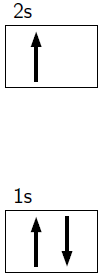
\includegraphics[width=.9cm]{col11305.imgs/m38741_CG10C3_009.png} % m38741;CG10C3\_009.png;;;6.0;8.5;
      \vspace{2pt}
    \vspace{\rubberspace}\par \begin{cnxcaption}
	  \small \textbf{Figure 3.13: }The electron configuration of Lithium, shown on an Aufbau diagram
	\end{cnxcaption}
    \vspace{.1in}
    \rule[.1in]{\figurerulewidth}{.005in} \\
    \end{center}
 \end{figure}       
        \label{m38741*id259749}A special type of notation is used to show an atom's electron configuration. The notation describes the energy levels, orbitals and the number of electrons in each. For example, the electron configuration of lithium is ${1\mathrm{s}}^{2}{2\mathrm{s}}^{1}$. The number and letter describe the energy level and orbital and the number above the orbital shows how many electrons are in that orbital.\par 
        \label{m38741*id259782}Aufbau diagrams for the elements fluorine and argon are shown in Figure~3.14 and Figure~3.15 respectively. Using standard notation, the electron configuration of fluorine is ${1\mathrm{s}}^{2}{2\mathrm{s}}^{2}{2\mathrm{p}}^{5}$ and the electron configuration of argon is ${1\mathrm{s}}^{2}{2\mathrm{s}}^{2}{2\mathrm{p}}^{6}$.\par 
    \setcounter{subfigure}{0}
	\begin{figure}[H] % horizontal\label{m38741*uid102}
    \begin{center}
    \rule[.1in]{\figurerulewidth}{.005in} \\
        \label{m38741*uid102!!!underscore!!!media}\label{m38741*uid102!!!underscore!!!printimage}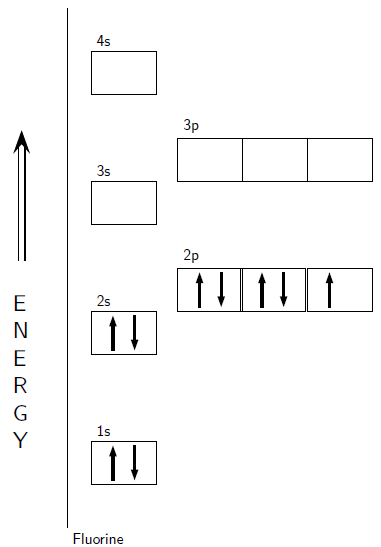
\includegraphics[height=300px]{col11305.imgs/m38741_CG10C3_010.png} % m38741;CG10C3\_010.png;;;6.0;8.5;
      \vspace{2pt}
    \vspace{\rubberspace}\par \begin{cnxcaption}
	  \small \textbf{Figure 3.14: }An Aufbau diagram showing the electron configuration of fluorine
	\end{cnxcaption}
    \vspace{.1in}
    \rule[.1in]{\figurerulewidth}{.005in} \\
    \end{center}
 \end{figure}       
    \setcounter{subfigure}{0}
	\begin{figure}[H] % horizontal\label{m38741*uid103}
    \begin{center}
    \rule[.1in]{\figurerulewidth}{.005in} \\
        \label{m38741*uid103!!!underscore!!!media}\label{m38741*uid103!!!underscore!!!printimage}\includegraphics[height=300px]{col11305.imgs/m38741_CG10C3_011.png} % m38741;CG10C3\_011.png;;;6.0;8.5;
      \vspace{2pt}
    \vspace{\rubberspace}\par \begin{cnxcaption}
	  \small \textbf{Figure 3.15: }An Aufbau diagram showing the electron configuration of argon
	\end{cnxcaption}
    \vspace{.1in}
    \rule[.1in]{\figurerulewidth}{.005in} \\
    \end{center}
 \end{figure}       
      \par
            \label{m38741*eip-138}\vspace{.5cm} 
      \noindent
      \hspace*{-30pt}\includegraphics[width=0.5in]{col11305.imgs/pspencil2.png}   \raisebox{25mm}{   
      \begin{mdframed}[linewidth=4, leftmargin=40, rightmargin=40]  
      \begin{exercise}
    \noindent\textbf{Exercise 3.7: Aufbau diagrams}\label{m38741*eip-483}
  \label{m38741*eip-491}Give the electron configuration for sodium ($Na$) and draw an aufbau diagram.
  \par 
\vspace{5pt}
\label{m38741*eip-119}\noindent\textbf{Solution to Exercise }
\label{m38741*listfhsst!!!underscore!!!id667}\begin{enumerate}[noitemsep, label=\textbf{Step} \textbf{\arabic*}. ] 
            \leftskip=20pt\rightskip=\leftskip\item Sodium has 11 electrons.\item We start by placing two electrons in the $1s$ orbital: ${1s}^{2}$. Now we have 9 electrons left to place in orbitals, so we put two in the $2s$ orbital: ${2s}^{2}$. There are now 7 electrons to place in orbitals so we place 6 of them in the $2p$ orbital: ${2p}^{6}$. The last electron goes into the $3s$ orbital: ${3s}^{1}$.\item The electron configuration is: ${1s}^{2}{2s}^{2}{2p}^{6}{3s}^{1}$\item Using the electron configuration we get the following diagram:
    \setcounter{subfigure}{0}
	\begin{figure}[H] % horizontal\label{m38741*uid847}
    \begin{center}
    \label{m38741*uid847!!!underscore!!!media}\label{m38741*uid847!!!underscore!!!printimage}\includegraphics[width=3cm]{col11305.imgs/m38126_wexaufbau.png} % ;wexaufbau.png;;;6.0;8.5;
      \vspace{2pt}
    \vspace{.1in}
    \end{center}
 \end{figure}       \end{enumerate}
    \end{exercise}
    \end{mdframed}
    }
    \noindent
  \label{m38741*eip-793}There are different orbital shapes, but we will be mainly dealing with only two. These are the 's' and 'p' orbitals (there are also 'd' and 'f' orbitals). The 's' orbitals are spherical and the 'p' orbitals are dumbbell shaped. 
    \setcounter{subfigure}{0}
	\begin{figure}[H] % horizontal\label{m38741*id8245}
    \begin{center}
    \label{m38741*uid8934!!!underscore!!!media}\label{m38741*uid8934!!!underscore!!!printimage}\includegraphics[width=5cm]{col11305.imgs/m38741_orbitals.png} % m38741;orbitals.png;;;6.0;8.5;
      \vspace{2pt}
    \vspace{\rubberspace}\par \begin{cnxcaption}
	  \small \textbf{Figure 3.17: }The shapes of orbitals. a) shows an 's' orbital, b) shows a single 'p' orbital and c) shows the three 'p' orbitals.
	\end{cnxcaption}
    \vspace{.1in}
    \end{center}
 \end{figure}       \par \label{m38741*eip-581}
            \subsubsection{ Hund's rule and Pauli's principle}
            \nopagebreak
            \label{m38741*eip-188}
Sometimes people refer to Hund's rule for electron configuration. This rule simply says that electrons would rather be in a subshell on their own than share a subshell. This is why when you are filling the subshells you put one electron in each subshell and then go back and fill the subshell, before moving onto the next energy level.
\par 
\label{m38741*eip-id1167385514309}
Pauli's exclusion principle simply states that electrons have a property known as spin and that two electrons in a subshell will not spin the same way. This is why we draw electrons as one arrow pointing up and one arrow pointing down.
\par \label{m38741*uid104}
            \subsubsection{ Core and valence electrons}
            \nopagebreak
        \label{m38741*id259935}Electrons in the outermost energy level of an atom are called \textbf{valence electrons}. The electrons that are in the energy shells closer to the nucleus are called \textbf{core electrons}. Core electrons are all the electrons in an atom, excluding the valence electrons. An element that has its valence energy level full is \textsl{more stable} and \textsl{less likely to react} than other elements with a valence energy level that is not full.\par 
\label{m38741*fhsst!!!underscore!!!id755}\begin{definition}
	  \begin{tabular*}{15 cm}{m{15 mm}m{}}
	\hspace*{-50pt}  \includegraphics[width=0.5in]{col11305.imgs/psflag2.png}   & \Definition{   \label{id2421518}\textbf{ Valence electrons }} { \label{m38741*meaningfhsst!!!underscore!!!id755}
        \label{m38741*id259971}The electrons in the outer energy level of an atom \par 
         } 
      \end{tabular*}
      \end{definition}
\label{m38741*fhsst!!!underscore!!!id758}\begin{definition}
	  \begin{tabular*}{15 cm}{m{15 mm}m{}}
	\hspace*{-50pt}  \includegraphics[width=0.5in]{col11305.imgs/psflag2.png}   & \Definition{   \label{id2421542}\textbf{ Core electrons }} { \label{m38741*meaningfhsst!!!underscore!!!id758}
        \label{m38741*id259989}All the electrons in an atom, excluding the valence electrons \par 
         } 
      \end{tabular*}
      \end{definition}
      \label{m38741*uid105}
            \subsubsection{ The importance of understanding electron configuration}
            \nopagebreak
        \label{m38741*id260011}By this stage, you may well be wondering why it is important for you to understand how electrons are arranged around the nucleus of an atom. Remember that during chemical reactions, when atoms come into contact with one another, it is the \textsl{electrons} of these atoms that will interact first. More specifically, it is the \textbf{valence electrons} of the atoms that will determine how they react with one another.\par 
        \label{m38741*id260029}To take this a step further, an atom is at its most stable (and therefore \textsl{unreactive}) when all its orbitals are full. On the other hand, an atom is least stable (and therefore most \textsl{reactive}) when its valence electron orbitals are not full. This will make more sense when we go on to look at chemical bonding in a later chapter. To put it simply, the valence electrons are largely responsible for an element's chemical behaviour and elements that have the same number of valence electrons often have similar chemical properties.\par 
\label{m38741*eip-106}One final point to note about electron configurations is stability. Which configurations are stable and which are not? Very simply, the most stable configurations are the ones that have full energy levels. These configurations occur in the noble gases. The noble gases are very stable elements that do not react easily (if at all) with any other elements. This is due to the full energy levels. All elements would like to reach the most stable electron configurations, i.e. all elements want to be noble gases. This principle of stability is sometimes referred to as the octet rule. An octet is a set of 8, and the number of electrons in a full energy level is 8. \par \label{m38741*eip-739}
            \subsubsection{ Experiment: Flame tests}
            \nopagebreak
            \label{m38741*eip-699}\noindent{}\textbf{Aim:}\newline
    To determine what colour a metal cation will cause a flame to be.
\par 
\label{m38741*eip-6991}\noindent{}\textbf{Apparatus:}\newline
    Watch glass, bunsen burner, methanol, bamboo sticks, metal salts (e.g. $\mathrm{NaCl}$, ${\mathrm{CuCl}}_{2}$, ${\mathrm{CaCl}}_{2}$, $\mathrm{KCl}$, etc. ) and metal powders (e.g. copper, magnesium, zinc, iron, etc.)
\par 
\label{m38741*eip-479}
\begin{tabular}{cc}
	\hspace*{-50pt}\raisebox{-8 mm}{\hspace{-0.2in}\includegraphics[width=0.75in]{col11305.imgs/psfact2.png} } & 
	\begin{minipage}{0.85\textwidth}
	\begin{note}
      {warning: }Be careful when working with bunsen burners as you can easily burn yourself. Make sure all scarves/loose clothing is securely tucked in and long hair is tied back. Ensure that you work in a well-ventilated space and that there is nothing flammable near the open flame.
	\end{note}
	\end{minipage}
	\end{tabular}
	\par
      \label{m38741*eip-6992}\noindent{}\textbf{Method:}\newline
    For each salt or powder do the following: \label{m38741*id7092}\begin{enumerate}[noitemsep, label=\textbf{\arabic*}. ] 
            \item Dip a clean bamboo stick into the methanol\item Dip the stick into the salt or powder\item Wave the stick through the flame from the bunsen burner. DO NOT hold the stick in the flame, but rather wave it back and forth through the flame.\item Observe what happens\end{enumerate}
\par 
\label{m38741*eip-6993}\noindent{}\textbf{Results:}\newline
    Record your results in a table, listing the metal salt and the colour of the flame.
\par 
\label{m38741*eip-6994}\noindent{}\textbf{Conclusion:}\newline
    You should have observed different colours for each of the metal salts and powders that you tested.\par \label{m38741*eip-378}The above experiment on flame tests relates to the line emission spectra of the metals. These line emission spectra are a direct result of the arrangement of the electrons in metals.\par \label{m38741*secfhsst!!!underscore!!!id766}
            \subsubsection{  Energy diagrams and electrons
        }
            \nopagebreak
        \label{m38741*id260063}\begin{enumerate}[noitemsep, label=\textbf{\arabic*}. ] 
            \label{m38741*uid106}\item Draw Aufbau diagrams to show the electron configuration of each of the following elements:
\label{m38741*id260079}\begin{enumerate}[noitemsep, label=\textbf{\alph*}. ] 
            \label{m38741*uid107}\item magnesium
\label{m38741*uid108}\item potassium
\label{m38741*uid109}\item sulphur
\label{m38741*uid110}\item neon
\label{m38741*uid111}\item nitrogen
\end{enumerate}
        \label{m38741*uid112}\item Use the Aufbau diagrams you drew to help you complete the following table:
    % \textbf{m38741*id260157}\par
          \begin{table}[H]
    % \begin{table}[H]
    % \\ 'id2891050' '1'
        \begin{center}
      \label{m38741*id260157}
    \noindent
    \tabletail{%
        \hline
        \multicolumn{5}{|p{\mytableboxwidth}|}{\raggedleft \small \sl continued on next page}\\
        \hline
      }
      \tablelasttail{}
      \begin{xtabular}[t]{|l|l|l|l|l|}\hline
        \textbf{Element} &
        \textbf{No. of energy levels} &
        \textbf{No. of core electrons} &
        \textbf{No. of valence electrons} &
        \textbf{Electron configuration (standard notation)}% make-rowspan-placeholders
     \tabularnewline\cline{1-1}\cline{2-2}\cline{3-3}\cline{4-4}\cline{5-5}
      %--------------------------------------------------------------------
        $\mathrm{Mg}$ &
         &
         &
         &
        % make-rowspan-placeholders
     \tabularnewline\cline{1-1}\cline{2-2}\cline{3-3}\cline{4-4}\cline{5-5}
      %--------------------------------------------------------------------
        $\mathrm{K}$ &
         &
         &
         &
        % make-rowspan-placeholders
     \tabularnewline\cline{1-1}\cline{2-2}\cline{3-3}\cline{4-4}\cline{5-5}
      %--------------------------------------------------------------------
        $\mathrm{S}$ &
         &
         &
         &
        % make-rowspan-placeholders
     \tabularnewline\cline{1-1}\cline{2-2}\cline{3-3}\cline{4-4}\cline{5-5}
      %--------------------------------------------------------------------
        $\mathrm{Ne}$ &
         &
         &
         &
        % make-rowspan-placeholders
     \tabularnewline\cline{1-1}\cline{2-2}\cline{3-3}\cline{4-4}\cline{5-5}
      %--------------------------------------------------------------------
        $\mathrm{N}$ &
         &
         &
         &
        % make-rowspan-placeholders
     \tabularnewline\cline{1-1}\cline{2-2}\cline{3-3}\cline{4-4}\cline{5-5}
      %--------------------------------------------------------------------
    \end{xtabular}
      \end{center}
    \begin{center}{\small\bfseries Table 3.8}\end{center}
    \begin{caption}{\small\bfseries Table 3.8}\end{caption}
\end{table}
    \par
  \label{m38741*uid113}\item Rank the elements used above in order of \textsl{increasing reactivity}. Give reasons for the order you give.
 Click here for the answer\footnote{http://www.fhsst.org/ll2}
        \end{enumerate}
\label{m38741*secfhsst!!!underscore!!!id783}
            \subsubsection{ Group work : Building a model of an atom         }
            \nopagebreak
            \label{m38741*id260472}Earlier in this chapter, we talked about different 'models' of the atom. In science, one of the uses of models is that they can help us to understand the structure of something that we can't see. In the case of the atom, models help us to build a picture in our heads of what the atom looks like.\par 
        \label{m38741*id260480}Models are often simplified. The small toy cars that you may have played with as a child are models. They give you a good idea of what a real car looks like, but they are much smaller and much simpler. A model cannot always be absolutely accurate and it is important that we realise this so that we don't build up a false idea about something.\par 
        \label{m38741*id260488}In groups of 4-5, you are going to build a model of an atom. Before you start, think about these questions:\par 
        \label{m38741*id260495}\begin{itemize}[noitemsep]
            \label{m38741*uid114}\item What information do I know about the structure of the atom? (e.g. what parts make it up? how big is it?)
\label{m38741*uid115}\item What materials can I use to represent these parts of the atom as accurately as I can?
\label{m38741*uid116}\item How will I put all these different parts together in my model?
\end{itemize}
        \label{m38741*id260537}As a group, share your ideas and then plan how you will build your model. Once you have built your model, discuss the following questions:\par 
        \label{m38741*id260542}\begin{itemize}[noitemsep]
            \label{m38741*uid117}\item Does our model give a good idea of what the atom actually looks like?
\label{m38741*uid118}\item In what ways is our model \textsl{inaccurate}? For example, we know that electrons \textsl{move} around the atom's nucleus, but in your model, it might not have been possible for you to show this.
\label{m38741*uid119}\item Are there any ways in which our model could be improved?
\end{itemize}
        \label{m38741*id260596}Now look at what other groups have done. Discuss the same questions for each of the models you see and record your answers. \par 
      \label{m38741*eip-816}The following simulation allows you to build an atom\newline
    \setcounter{subfigure}{0}
	\begin{figure}[H] % horizontal\label{m38806*transverse-waves}
    \textnormal{Phet simulation for building atoms}\vspace{.1in} \nopagebreak
  \label{m38806*phet!!!underscore!!!sim}\label{m38806*phet-simulation}
            \raisebox{-5 pt}{ \includegraphics[width=0.5cm]{col11305.imgs/summary_www.png}} { (Simulation:  lbb )}
      \vspace{2pt}
    \vspace{.1in}
 \end{figure}       
\par \label{m38741*eip-583}This is another simulation that allows you to build an atom. This simulation also provides a summary of what you have learnt so far. \newline
    \setcounter{subfigure}{0}
	\begin{figure}[H] % horizontal\label{m38806*transverse-waves}
    \textnormal{Simulation for building atoms 2}\vspace{.1in} \nopagebreak
  \label{m38806*phet!!!underscore!!!sim}\label{m38806*phet-simulation}
            \raisebox{-5 pt}{ \includegraphics[width=0.5cm]{col11305.imgs/summary_www.png}} { (Simulation:  lbj )}
      \vspace{2pt}
    \vspace{.1in}
 \end{figure}       
    \par 
    \label{m38741*cid10}
            \subsection{ Summary}
            \nopagebreak
      \label{m38741*id262657}\begin{itemize}[noitemsep]
            \label{m38741*uid169}\item Much of what we know today about the atom, has been the result of the work of a number of scientists who have added to each other's work to give us a good understanding of atomic structure.
\label{m38741*uid170}\item Some of the important scientific contributors include \textbf{J.J.Thomson} (discovery of the electron, which led to the Plum Pudding Model of the atom), \textbf{Ernest Rutherford} (discovery that positive charge is concentrated in the centre of the atom) and \textbf{Niels Bohr} (the arrangement of electrons around the nucleus in energy levels).
\label{m38741*uid171}\item Because of the very small mass of atoms, their mass is measured in \textbf{atomic mass units} (u). $1\phantom{\rule{2pt}{0ex}}u=1,67\ensuremath{\times}10{}^{-24}\phantom{\rule{2pt}{0ex}}g$.
\label{m38741*uid172}\item An atom is made up of a central \textbf{nucleus} (containing \textbf{protons} and \textbf{neutrons}), surrounded by \textbf{electrons}.
\label{m38741*uid173}\item The \textbf{atomic number} (Z) is the number of protons in an atom.
\label{m38741*uid174}\item The \textbf{atomic mass number} (A) is the number of protons and neutrons in the nucleus of an atom.
\label{m38741*uid175}\item The \textbf{standard notation} that is used to write an element, is $_{Z}^{A}\mathrm{X}$, where X is the element symbol, A is the atomic mass number and Z is the atomic number.
\label{m38741*uid176}\item The \textbf{isotope} of a particular element is made up of atoms which have the same number of protons as the atoms in the original element, but a different number of neutrons. This means that not all atoms of an element will have the same atomic mass.
\label{m38741*uid177}\item The \textbf{relative atomic mass} of an element is the average mass of one atom of all the naturally occurring isotopes of a particular chemical element, expressed in atomic mass units. The relative atomic mass is written under the elements' symbol on the Periodic Table.
\label{m38741*uid178}\item The energy of electrons in an atom is \textbf{quantised}. Electrons occur in specific energy levels around an atom's nucleus.
\label{m38741*uid179}\item Within each energy level, an electron may move within a particular shape of \textbf{orbital}. An orbital defines the space in which an electron is most likely to be found. There are different orbital shapes, including s, p, d and f orbitals.
\label{m38741*uid180}\item Energy diagrams such as \textbf{Aufbau diagrams} are used to show the electron configuration of atoms.
\label{m38741*uid181}\item The electrons in the outermost energy level are called \textbf{valence electrons}.
\label{m38741*uid182}\item The electrons that are not valence electrons are called \textbf{core electrons}.
\label{m38741*uid183}\item Atoms whose outermost energy level is full, are less chemically reactive and therefore more stable, than those atoms whose outer energy level is not full.
\end{itemize}
\label{m38741*eip-867}
    \setcounter{subfigure}{0}
	\begin{figure}[H] % horizontal\label{m38741*slidesharefigure2}
    \label{m38741*slidesharemedia2}\label{m38741*slideshareflash2}
            \raisebox{-5 pt}{ \includegraphics[width=0.5cm]{col11305.imgs/summary_www.png}} { (Presentation:  P10024 )}
      \vspace{2pt}
    \vspace{.1in}
 \end{figure}       \par \label{m38741*secfhsst!!!underscore!!!id1140}
            \subsubsection{ End of chapter exercises}
            \nopagebreak
      \label{m38741*id263110}\begin{enumerate}[noitemsep, label=\textbf{\arabic*}. ] 
            \label{m38741*uid189}\item Write down only the word/term for each of the following descriptions.
\label{m38741*id263126}\begin{enumerate}[noitemsep, label=\textbf{\alph*}. ] 
            \label{m38741*uid190}\item The sum of the number of protons and neutrons in an atom
\label{m38741*uid191}\item The defined space around an atom's nucleus, where an electron is most likely to be found
\end{enumerate}
                \label{m38741*uid192}\item For each of the following, say whether the statement is True or False. If it is False, re-write the statement correctly.
\label{m38741*id263169}\begin{enumerate}[noitemsep, label=\textbf{\alph*}. ] 
            \label{m38741*uid193}\item $_{10}^{20}\mathrm{Ne}$ and $_{10}^{22}\mathrm{Ne}$ each have 10 protons, 12 electrons and 12 neutrons.
\label{m38741*uid194}\item The atomic mass of any atom of a particular element is always the same.
\label{m38741*uid195}\item It is safer to use helium gas rather than hydrogen gas in balloons.
\label{m38741*uid196}\item Group 1 elements readily form negative ions.
\end{enumerate}
                \label{m38741*uid197}\item Multiple choice questions: In each of the following, choose the \textbf{one} correct answer.
\label{m38741*id263273}\begin{enumerate}[noitemsep, label=\textbf{\alph*}. ] 
            \label{m38741*uid198}\item The three basic components of an atom are:
\label{m38741*id263289}\begin{enumerate}[noitemsep, label=\textbf{\alph*}. ] 
            \label{m38741*uid199}\item protons, neutrons, and ions
\label{m38741*uid200}\item protons, neutrons, and electrons
\label{m38741*uid201}\item protons, neutrinos, and ions
\label{m38741*uid202}\item protium, deuterium, and tritium
\end{enumerate}
                \label{m38741*uid203}\item The charge of an atom is...
\label{m38741*id263355}\begin{enumerate}[noitemsep, label=\textbf{\alph*}. ] 
            \label{m38741*uid204}\item positive
\label{m38741*uid205}\item neutral
\label{m38741*uid206}\item negative
\end{enumerate}
                \label{m38741*uid207}\item If Rutherford had used neutrons instead of alpha particles in his scattering experiment, the neutrons would...
\label{m38741*id263410}\begin{enumerate}[noitemsep, label=\textbf{\alph*}. ] 
            \label{m38741*uid208}\item not deflect because they have no charge
\label{m38741*uid209}\item have deflected more often
\label{m38741*uid210}\item have been attracted to the nucleus easily
\label{m38741*uid211}\item have given the same results
\end{enumerate}
                \label{m38741*uid212}\item Consider the isotope $_{92}^{234}\mathrm{U}$. Which of the following statements is \textsl{true}?
\label{m38741*id263500}\begin{enumerate}[noitemsep, label=\textbf{\alph*}. ] 
            \label{m38741*uid213}\item The element is an isotope of $_{94}^{234}\mathrm{Pu}$
\label{m38741*uid214}\item The element contains 234 neutrons
\label{m38741*uid215}\item The element has the same electron configuration as $_{92}^{238}\mathrm{U}$
\label{m38741*uid216}\item The element has an atomic mass number of 92
\end{enumerate}
                \label{m38741*uid217}\item The electron configuration of an atom of chlorine can be represented using the following notation:
\label{m38741*id263598}\begin{enumerate}[noitemsep, label=\textbf{\alph*}. ] 
            \label{m38741*uid218}\item  ${1\mathrm{s}}^{2}{2\mathrm{s}}^{8}{3\mathrm{s}}^{7}$\label{m38741*uid219}\item 
${1\mathrm{s}}^{2}{2\mathrm{s}}^{2}{2\mathrm{p}}^{6}{3\mathrm{s}}^{2}{3\mathrm{p}}^{5}$
\label{m38741*uid220}\item 
${1\mathrm{s}}^{2}{2\mathrm{s}}^{2}{2\mathrm{p}}^{6}{3\mathrm{s}}^{2}{3\mathrm{p}}^{6}$\label{m38741*uid221}\item 
${1\mathrm{s}}^{2}{2\mathrm{s}}^{2}{2\mathrm{p}}^{5}$\end{enumerate}
                \end{enumerate}
        \item Give the standard notation for the following elements:
\label{m38741*id8223}\begin{enumerate}[noitemsep, label=\textbf{\alph*}. ] 
            \item beryllium\item carbon-12\item titanium-48\item fluorine\end{enumerate}
\item Give the electron configurations and aufbau diagrams for the following elements:\label{m38741*id7624}\begin{enumerate}[noitemsep, label=\textbf{\alph*}. ] 
            \item aluminium\item phosphorus\item carbon\end{enumerate}
\item Use standard notation to represent the following elements: \label{m38741*id74324}\begin{enumerate}[noitemsep, label=\textbf{\alph*}. ] 
            \item argon\item calcium\item silver-107\item bromine-79\end{enumerate}
\item For each of the following elements give the number of protons, neutrons and electrons in the element: \label{m38741*id74374}\begin{enumerate}[noitemsep, label=\textbf{\alph*}. ] 
            \item $_{78}^{195}\mathrm{Pt}$\item $_{18}^{40}\mathrm{Ar}$\item $_{27}^{59}\mathrm{Co}$\item $_{3}^{7}\mathrm{Li}$\item $_{5}^{11}\mathrm{B}$\end{enumerate}
\item For each of the following elements give the element or number represented by 'x': \label{m38741*id7434324}\begin{enumerate}[noitemsep, label=\textbf{\alph*}. ] 
            \item $_{45}^{103}\mathrm{X}$\item $_{x}^{35}\mathrm{Cl}$\item $_{4}^{x}\mathrm{Be}$\end{enumerate}
\item Which of the following are isotopes of $_{12}^{24}\mathrm{Mg}$: \label{m38741*id743234}\begin{enumerate}[noitemsep, label=\textbf{\alph*}. ] 
            \item $_{25}^{12}\mathrm{Mg}$\item $_{12}^{26}\mathrm{Mg}$\item $_{13}^{24}\mathrm{Al}$\end{enumerate}
\item If a sample contains 69\% of copper-63 and 31\% of copper-65, calculate the relative atomic mass of an atom in that sample.\newline
            \item Complete the following table:
    % \textbf{m38741*eip-282}\par
          \begin{table}[H]
    % \begin{table}[H]
    % \\ 'id2892806' '1'
        \begin{center}
      \label{m38741*eip-282}
    \noindent
    \tabletail{%
        \hline
        \multicolumn{4}{|p{\mytableboxwidth}|}{\raggedleft \small \sl continued on next page}\\
        \hline
      }
      \tablelasttail{}
      \begin{xtabular}[t]{|l|l|l|l|}\hline
        Element &
        Electron configuration &
        Core electrons &
        Valence electrons% make-rowspan-placeholders
     \tabularnewline\cline{1-1}\cline{2-2}\cline{3-3}\cline{4-4}
      %--------------------------------------------------------------------
        Boron (B) &
         &
         &
        % make-rowspan-placeholders
     \tabularnewline\cline{1-1}\cline{2-2}\cline{3-3}\cline{4-4}
      %--------------------------------------------------------------------
        Calcium (Ca) &
         &
         &
        % make-rowspan-placeholders
     \tabularnewline\cline{1-1}\cline{2-2}\cline{3-3}\cline{4-4}
      %--------------------------------------------------------------------
        Silicon (Si) &
         &
         &
        % make-rowspan-placeholders
     \tabularnewline\cline{1-1}\cline{2-2}\cline{3-3}\cline{4-4}
      %--------------------------------------------------------------------
        Lithium (Li) &
         &
         &
        % make-rowspan-placeholders
     \tabularnewline\cline{1-1}\cline{2-2}\cline{3-3}\cline{4-4}
      %--------------------------------------------------------------------
        Neon (Ne) &
         &
         &
        % make-rowspan-placeholders
     \tabularnewline\cline{1-1}\cline{2-2}\cline{3-3}\cline{4-4}
      %--------------------------------------------------------------------
    \end{xtabular}
      \end{center}
    \begin{center}{\small\bfseries Table 3.9}\end{center}
    \begin{caption}{\small\bfseries Table 3.9}\end{caption}
\end{table}
    \par
\item Draw aufbau diagrams for the following elements:\label{m38741*id78624}\begin{enumerate}[noitemsep, label=\textbf{\alph*}. ] 
            \item beryllium\item sulphur\item argon\end{enumerate}
\end{enumerate}
  \label{m38741**end}
  \label{ea1c9e59656f96ee804546971cf6dee6**end}
\par \raisebox{-5 pt}{\includegraphics[width=0.5cm]{col11305.imgs/summary_www.png}} Find the answers with the shortcodes:
 \par \begin{tabular}[h]{cccccc}
 (1.) lif  &  (2.) liG  &  (3.) li7  &  (4.) liA  &  (5.) lio  &  (6.) lis  &  (7.) liH  &  (8.) lg7  &  (9.) lgG  &  (10.) l44  &  (11.) l42  &  (12.) l4T  &  (13.) l4b  &  (14.) l4j  &  (15.) l4D  &  (16.) lgW  & \end{tabular}
